\documentclass[11pt]{article}

\usepackage[italian]{babel}

\usepackage[utf8]{inputenc} % Required for inputting international characters
\usepackage[T1]{fontenc} % Output font encoding for international characters

\usepackage{mathpazo} % Palatino font
\usepackage{graphicx}
\usepackage{fancyhdr}
\usepackage{tabularx}
\usepackage{geometry}

\geometry{legalpaper, margin=2.5cm}

\newcommand{\doctitle}{Requirement Analysis Document}
\newcommand{\docversion}{1.0}

\begin{document}
	
	%----------------------------------------------------------------------------------------
	%	TITLE PAGE
	%----------------------------------------------------------------------------------------
	
	\begin{titlepage} % Suppresses displaying the page number on the title page and the subsequent page counts as page 1
		\newcommand{\HRule}{\rule{\linewidth}{0.5mm}} % Defines a new command for horizontal lines, change thickness here
		
		\center % Centre everything on the page
		
		%------------------------------------------------
		%	Headings
		%------------------------------------------------
		
		\textsc{\LARGE Università degli Studi di Salerno}\\
		\textsc{\large Corso di Ingegneria del Software}\\[1.5cm] % Main heading such as the name of your university/college
		
		%------------------------------------------------
		%	Title
		%------------------------------------------------
		
		\HRule\\[0.4cm]
		
		{\huge\bfseries ASCETIC}\\ % Title of your document
		\vspace{0.2cm}
		{\large\bfseries Automated Code Smell Identification and Correction}\\[0.2cm] % Title of your document
		
		\HRule\\[1.5cm]
		
		\textsc{\Large \doctitle}\\[0.3cm] % Major heading such as course name
		
		\textsc{\large Version \docversion}\\[0.5cm] % Minor heading such as course title
		
		
		%------------------------------------------------
		%	Logo
		%------------------------------------------------
		
		\vfill\vfill
		
		
\includegraphics[width=0.5\textwidth]{logo_temp.jpg}\\[1cm] % Include a department/university logo - this will require the graphicx package
		
		%------------------------------------------------
		%	Date
		%------------------------------------------------
		
		\vfill\vfill\vfill % Position the date 3/4 down the remaining page
		
		{\large\today} % Date, change the \today to a set date if you want to be precise
		
		
		
		%----------------------------------------------------------------------------------------
		
		\vfill % Push the date up 1/4 of the remaining page
		
	\end{titlepage}
	
	%----------------------------------------------------------------------------------------
	
	\pagestyle{fancy}
	\rhead{ASCETIC}
	\lhead{\doctitle~v.~\docversion}
	\renewcommand{\headrulewidth}{0pt}	
	
	\textbf{Coordinatore Progetto:}
	\begin{table}[h]
		\centering
		\begin{tabularx}{0.9\textwidth}{|X|X|}
			\hline
			\textbf{Nome}     & \textbf{Matricola} \\ \hline
			Manuel De Stefano &  0522500633\\ \hline
		\end{tabularx}
	\end{table}
	
	\vspace{0.5cm}
	
	\textbf{Partecipanti:}
	\begin{table}[h]
		\centering
		\begin{tabularx}{0.9\textwidth}{|X|X|}
			\hline
			\textbf{Nome}     & \textbf{Matricola} \\ \hline
			Amoriello Nicola &  0512104742\\ \hline
			Di Dario Dario &  0512104758\\ \hline
			Gambardella Michele Simone &  0512104502\\ \hline
			Iovane Francesco &  0512104550\\ \hline
			Pascucci Domenico &  0512102950\\ \hline
			Patierno Sara &  0512103460\\ \hline
		\end{tabularx}
	\end{table}
	
	\textbf{Revision History:}
	\begin{table}[h]
		\centering
		\begin{tabularx}{0.9\textwidth}{|p{2cm}|l|X|p{3cm}|}
			\hline
			\textbf{Data} & \textbf{Versione} & \textbf{Descrizione} & \textbf{Autore} \\ \hline
			26/10/2018 & 1.0 & Prima stesura & Tutto il Team \\ \hline
		\end{tabularx}
	\end{table}
	
	\vfill
	\newpage
	
	\tableofcontents
	\newpage
	
	\section{Introduction}	   
	   		   
	   	\subsection{Scope of the system}
	   		Durante il ciclo di vita di un software i cambiamenti sono inevitabili.\\
	   		La manutenzione, che sia per correggere bug o per aggiungere nuove funzionalità, porta a un graduale deperimento del codice, il quale non inficia la correttezza del programma ma porta a debolezze di progettazione: i cosiddetti code smell.\\
	   		Anche uno sviluppatore navigato e ben attento a queste problematiche può cadere in errore, a causa di tempistiche strette o codice ripreso da altri developer.\\
	   	    ASCETIC nasce per permettere a utenti, esperti e non, di refactorizzare il codice in maniera comoda e intelligente.\\
	   		Il plug-in, sviluppato per l'IDE intelliJ IDEA, consente di analizzare il progetto, rilevando 4 possibili tipologie di smell(Blob, Promiscuous Package, Feature Envy, Missplaced Class) e di effettuare un eventuale correzione automatica.
	   		
	   	\subsection{Overview}
	   		ASCETIC (Inizialmente TACOR) è un'opera di reengineering, la quale ha l'obiettivo di migliorare le funzionalità già offerte dal precedente plug-in, offrirne delle nuove ed effettuare un restyling dell'interfaccia grafica per rendere migliore l'esperienza d'uso. ASCETIC si rivolge ad un pubblico composto principalmente da sviluppatori Java che utilizzano l'IDE IntelliJ IDEA e si pone l'obiettivo di facilitare l'aggiustamento del codice sorgente. Lo sviluppatore ha la possibilità di: 
	   		\begin{itemize}
	   			\item Applicare la correzione automatica proposta dal sistema dei Code Smell rilevati durante la fase d'analisi. E' possibile applicare tale soluzione a tutti gli elementi rilevati oppure ad uno specifico insieme selezionato dall'utente.
	   			\item Porre determinati Smell, scelti ad hoc dallo sviluppatore, come "falsi positivi", cosicché il sistema ignori quella determinata sezione di codice fino a nuova modifica. 
	   			\item Utilizzare la funzione "Reminder", la quale fornisce un comodo promemoria così da poter affrontare manualmente la correzione dello smell selezionato. 
	   		
	   		\end{itemize}
	   	
	   	
	   	\subsection{Definitions, acronyms, and abbreviations}
	   	
	   	Code Smell : Sezioni di codice scritte in maniera non ottimale, presentanti debolezze di progettazione che riducono la qualità del codice, non compromettendone il funzionamento.
	    \newline
	   	\\ASCETIC : acronimo per Automated Code Smell Identification and Correction. 
	   	
	\section{Current system}
	
			\subsection{Requisiti Funzionali}
		\paragraph{RF 1 - Ricerca code smell}  
		\begin{quote}Il sistema ricerca i code smell all'interno del codice java.	
			\begin{description}
				\item [RF 1.1:]Il sistema permette l'analisi di code smell di tipo Blob,
				\item [RF 1.2:]Il sistema permette l'analisi di code smell di tipo Misplaced Class
				\item [RF 1.3:]Il sistema permette l'analisi di code smell di tipo Feature Envy
				\item [RF 1.4:]Il sistema permette l'analisi di code smell di tipo Promiscuos Package
			\end{description}
		\end{quote}
		
		
		
		\paragraph{RF 2 - Correzione} 
		\begin{quote}Il sistema mostra una possibile soluzione al code smell.
			\begin{description}
				\item [RF 2.1:] Il sistema permette di corregere code smell di tipo Feature Envy.
				\item [RF 2.2:] Il sistema permette di corregere code smell di tipo Misplaced Class.
			\end{description}
		\end{quote}
		
		
		\paragraph{RF 3 - Refactoring} 
		\begin{quote}Il sistema permette allo sviluppatore di risolvere il code smell con degli automatismi del software.
			\begin{description}
				\item [RF 3.1:] Il sistema permette di risolvere code smell di tipo Feature Envy.
				\item [RF 3.2:] Il sistema permette di risolvere code smell di tipo Misplaced Class.
			\end{description}
		\end{quote}
		
		
		\paragraph{RF 4 - Metriche di Qualità} 
		\begin{quote}Il sistema permette di calcolare metriche di qualità.
			\begin{description}
				\item [RF 4.1:] Il sistema permette di calcolare metriche di qualità per i metodi.
				\item [RF 4.2:] Il sistema permette di calcolare metriche di qualità per le classi.
				\item [RF 4.3:] Il sistema permette di calcolare metriche di qualità per i package.
			\end{description}
		\end{quote}
		
		\paragraph{RF 5 - Estrazione dei Topic} 
		\begin{quote}Il sistema consente di estrarre i topic implementati.
		\end{quote}
	
		\paragraph{RF 6 - Verifica Correzione}
		\begin{quote}Il sistema consente di verificare la correttezza del codice.
		\end{quote}  
	
			
	\subsection{Requisiti Non Funzionali}
	
		\begin{list}{-}{}
			
			\item \textbf{RNF 1 - Performance}\newline 
			Il sistema è concepito come utilizzabile da singolo utente, con un'interazione diretta, il tempo di risposta varia in base all'analisi proposta.
			\newline 
			\item \textbf{RNF 2 - Robustezza}
			\newline  Il sistema allo stato attuale non soddisfa il requisito di robustezza.
			\newline
			\item \textbf{RNF 3 - Sicurezza}
			\newline Il sistema si presenta sufficientemente sicuro in quanto il suo ambiente d'azione è locale, quindi non vi è la necessità di protezione da minacce esterne.
			\newline 
			\item \textbf{RNF 4 - Usabilità}
			\newline Il sistema presenta bassi criteri di usabilità, data una scarna e poco intuitiva GUI.
			\newline 
			\item \textbf{RNF 5 - Manutenibilità}\newline 
			Il sistema non presenta alcun tipo di documentazione pregressa, oltre ad adottare scelte implementative poco adatte a tale scopo.
			\newline  
			\item \textbf{RNF 6 - Implementazione}
			\newline Il sistema è realizzato interamente in linguaggio Java, sia parte back-end che front-end.
			\newline 
			\item \textbf{RNF 7 - Affidabilità}
			\newline  Il sistema allo stato attuale non rispetta il requisito di affidabilità.
	  \end{list}
		\subsection{Use Case Model}		
			
			\begin{figure}[h!]
				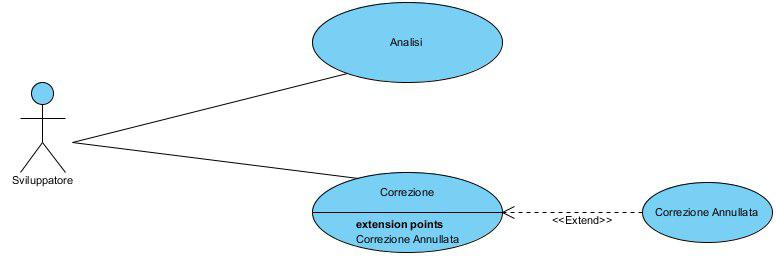
\includegraphics[width=\columnwidth]{UseCaseDiagramCurrent.jpg}
				\caption{UCD1-Analisi e Correzione}
			\end{figure}
		
			

		\begin{tabular}{|l|p{13cm}|}
			\hline
			\textbf{Use case name}  & \textbf{UC 1 - Ricerca di code smell} \\ \hline
			\textbf{Participating actors}  & \textbf{Sviluppatore} \\ \hline
			\textbf{Entry condition}  & L'utente avvia con successo Intellij.\\ \hline 			
			\textbf{Flow of events}  & 
			\begin{tabular}{p{6cm}p{6cm}p{6cm}}
				\centering\textbf{UTENTE}  & \centering\textbf{SISTEMA} &\\ \\
				\textbf{1.}\hspace{0.3cm}L'utente su IntelliJ, tramite menù a tendina del plug-in, richiede l'analisi locale sulla classe o sul package designato che vuole correggere, evidenziando che tipologia di code smell analizzare.\\ 
				&\textbf{2.}\hspace{0.3cm}Il sistema analizza il codice ed effettua il calcolo delle metriche strutturali. Sulla base dei dati estrapolati vengono poi mostrati i valori riguardanti le metriche di qualità.\\
				\textbf{3.}\hspace{0.3cm}L'utente prende visione del risultato dell'analisi tramite una tabella e varie RadarMap riportanti i 5 termini più frequenti . La tabella riporta la posizione del code smell identificato e le metriche di qualità calcolate(LOC, WNC, RFC, CBO, LCOM, NOA, NOM, NOPA, NOP). L'utente può inoltre, tramite apposito pulsante "Perform Refactor", richiedere il refactoring sullo smell. \\	\\		
			\end{tabular}\\ \hline		
			\textbf{Exit condition}  & Lo sviluppatore visiona correttamente i dati e il codice affetto da smell.\\ \hline 			
			\textbf{Exception condition} & Nel passo 1, in caso di codice java non corretto dal punto di vista sintattico, semantico o lessicale si verifica lo UC 1.1.\\ \hline
			\textbf{Priority}  & Alta \\ \hline 	
			\textbf{Quality requirements}  & 
					\begin{itemize}
						\item Tempo di elaborazione massimo: 3 minuti.
						\item Il sistema è in grado di rilevare se il codice è java.
					\end{itemize}
							
			\\ \hline 
		\end{tabular}

		\vspace{1cm}

		\begin{tabular}{|l|p{13cm}|}
			\hline
			\textbf{Use case name}  & \textbf{UC 1.1 - Analisi codice non compilabile} \\ \hline
			\textbf{Participating actors}  & \textbf{Sviluppatore} \\ \hline
			\textbf{Entry condition}  & L'utente avvia l'analisi del codice.\\ \hline 			
			\textbf{Flow of events}  & 
			\begin{tabular}{p{6cm}p{6cm}p{6cm}}
				\centering\textbf{UTENTE}  & \centering\textbf{SISTEMA} &\\ \\
				\textbf{1.}\hspace{0.3cm}L'utente attende l'elaborazioni richieste dal sistema.\\ 
				&\textbf{2.}\hspace{0.3cm}Il sistema tenta di analizzare il codice ma, trovando testo non compilabile, annulla l'operazione e mostra un messaggio di errore.\\
				\textbf{3.}\hspace{0.3cm}L'utente prende visione del messaggio che indica il fallimento dell'operazione. \\	\\		
			\end{tabular}\\ \hline		
			\textbf{Exit condition}  & Il sistema termina l'esecuzione senza effettuare alcuna modifica\\ \hline 			
			\textbf{Exception condition} & \\ \hline
			\textbf{Priority}  & Alta \\ \hline 	
			\textbf{Quality requirements}  & 
			\begin{itemize}
				\item Tempo di elaborazione massimo: 3 minuti.
			\end{itemize}
			
			\\ \hline 
		\end{tabular}
	
	 	\newpage 
	 	
			%USE CASE 2.1 - "CORREZIONE CODE SMELL SOLO FE"
		
		\begin{tabular}{|l|p{13cm}|}
			\hline
			\textbf{Use case name}  & \textbf{UC 2.1 - Correzione Code smell - Feature Envy} \\ \hline
			\textbf{Participating actors}  & \textbf{Sviluppatore} \\ \hline
			\textbf{Entry condition}  & L’utente ha visualizzato il codice affetto da smell  \\  \hline
			\textbf{Flow of events}  &  
			\begin{tabular}{p{6cm}p{6cm}p{6cm}}
				\centering \textbf{UTENTE} & \centering \textbf{SISTEMA} & \\
				\textbf{1.}\hspace{0.3cm}L’utente, dopo aver preso visione dei risultati dati del caso UC1.0 sceglie i parametri su cui intervenire per lo smells di tipo “Feature Envy” e avvia gli automatismi per la correzione automatica premendo il tasto “Refactor”.
				\\ \\ &
				\textbf{2.}\hspace{0.3cm}Il sistema, mostra una schermata di riepilogo con delle sezioni mostranti una proposta di correzione   confrontata con la situazione precedente all’analisi, e un tasto per apportare tali modifiche. \\ \\
				
				\textbf{3.}\hspace{0.3cm}L’utente, può scegliere di accettare tali modifiche consigliate dal sistema cliccando il tasto "Applica modifiche".
				\\ \\ &
				\textbf{4.}\hspace{0.3cm}Il sistema, applica la soluzione che precedentemente ha mostrato all'utente. \\ \\
				
				\textbf{5.}\hspace{0.3cm}L'utente prende visione di tutte le modifiche effettuate dal sistema. \\ \\
				
			\end{tabular}\\ \hline
			
						\textbf{Exit condition}  & Il codice è stato correttamente modificato.\\ \hline 
			\textbf{Exception condition} &Se nel passo 1 o 3 l'utente chiude la finestra di dialogo e non procede alla correzione si verifica lo UC 2.3\\ \hline
			\textbf{Priority}  & Alta \\ \hline 	
			\textbf{Quality requirements}  & 
			\\ \hline 
		\end{tabular}
		
		%USE CASE 2.2 - "CORREZIONE CODE SMELL SOLO MC"
		
		\begin{tabular}{|l|p{13cm}|}
			\hline
			\textbf{Use case name}  & \textbf{UC 2.2 - Correzione Code smell - Misplaced Class} \\ \hline
			\textbf{Participating actors}  & \textbf{Sviluppatore} \\ \hline
			\textbf{Entry condition}  & L’utente ha visualizzato il codice affetto da smell  \\  \hline
			\textbf{Flow of events}  &  
			\begin{tabular}{p{6cm}p{6cm}p{6cm}}
				\centering \textbf{UTENTE} & \centering \textbf{SISTEMA} & \\
				\textbf{1.}\hspace{0.3cm}L’utente, dopo aver preso visione dei risultati dati del caso UC1.0 sceglie i parametri su cui intervenire per lo smells di tipo “Misplaced Class” e avvia gli automatismi per la correzione automatica premendo il tasto “Refactor”.
				\\ \\ &
				\textbf{2.}\hspace{0.3cm}Il sistema, mostra una schermata di riepilogo con delle sezioni mostranti una proposta di correzione   confrontata con la situazione precedente all’analisi, e un tasto per apportare tali modifiche. \\ \\
				
				\textbf{3.}\hspace{0.3cm}L’utente, può scegliere di accettare tali modifiche consigliate dal sistema cliccando il tasto "Applica modifiche".
				\\ \\ &
				\textbf{4.}\hspace{0.3cm}Il sistema, applica la soluzione che precedentemente ha mostrato all'utente. \\ \\
				
				\textbf{5.}\hspace{0.3cm}L'utente prende visione di tutte le modifiche effettuate dal sistema. \\ \\
				
			\end{tabular}\\ \hline
			
			\textbf{Exit condition}  & Il codice è stato correttamente modificato.\\ \hline 
			\textbf{Exception condition} &Se nel passo 1 o 3 l'utente chiude la finestra di dialogo e non procede alla correzione si verifica lo UC 2.3\\ \hline
			\textbf{Priority}  & Alta \\ \hline 	
			\textbf{Quality requirements}  & 
			\\ \hline 
		\end{tabular}			
		
		\vspace{1cm} 
		
		\begin{tabular}{|l|p{13cm}|}
			\hline
			\textbf{Use case name}  & \textbf{UC 2.3 - Correzione annullata} \\ \hline
			\textbf{Participating actors} & \textbf{Sviluppatore} \\ \hline
			\textbf{Entry Condition} & L'utente chiude le finestre di dialogo e non procede alla correzione. \\ \hline
			\textbf{Flow of events} & 
			\begin{tabular}{p{6cm}p{6cm}p{6cm}}
				\centering \textbf{UTENTE} & \centering \textbf{SISTEMA} & \\
				\textbf{1.}\hspace{0.3cm}Lo Sviluppatore decide di non correggere il code smell. & \\
				& \textbf{2.}\hspace{0.3cm}Il Sistema non effettua alcuna operazione e vengono chiuse le finestre di dialogo. 
			\end{tabular} \\ \hline 
			\textbf{Exit condition} & Il Sistema termina l'operazione senza effettuare modifiche al codice.\\ \hline 
			\textbf{Exception condition} & \textbf{} \\ \hline
			\textbf{Priority}  & Alta \\ \hline 	
			\textbf{Quality requirements} & \textbf{} \\ \hline
		\end{tabular}
		
%\\sorgente, tipo, metriche  \\ \\	
		
		\subsection{Static Analysis Model}
		
			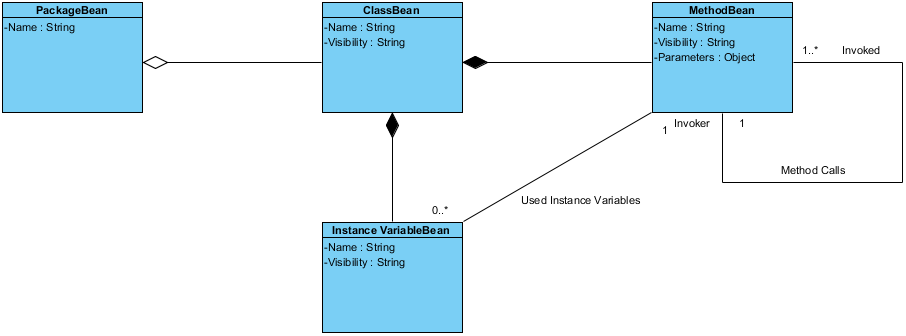
\includegraphics[width=\columnwidth]{classDiagram.png}
			
			
		\flushleft	

			\begin{tabular} {|l|p{3.5cm}|p{11cm}|}
					\hline \textbf{TIPO} & \textbf{NOME} & \textbf{DESCRIZIONE} \\ \hline
					Boundary & Search & Boundary che si occupa della riproduzione a schermo dei risultati dell'analisi. \\ 
					& Smell List & Boundary che si occupa della visualizzazione della lista degli smell trovati in fase di analisi. \\
					& Solution & Boundary che rende possibile visualizzare la lista delle soluzioni elaborate dal sistema. \\ 
					& Result & Boundary che rende possibile visualizzare i risultati dopo l'esecuzione del Refactor. \\ \hline
					Control & Search & Control che invia messaggi al Search Entity per ricercare smell ed istanzia lo Smell List Boundary, al quale invia un messaggio per richiedere la visualizzazione della lista degli smell.\\ 
					& Proposed Solution & Control che crea il Solution Boundary, al quale invia un messaggio per visualizzare le proposte di correzione. \\
					& Refactoring & Control che crea il Result Boundary, al quale invia un messaggio per notificare il successo dell'operazione di Refactoring. \\ \hline 
					Entity & Search & Entity che conserva i dati persistenti relativi ai Code Smell trovati in fase di analisi. \\ \hline
			\end{tabular}
			
			\vspace{0.5cm}
			
			\flushleft Gli oggetti presenti nella tabella soprastante sono stati individuati a seguito dell'analisi dinamica sotto riportata.  
			
			\vspace{0.5cm}
			\newpage				
		\subsection{Dynamic Analysis Model}
		
		
	
		
			\subsubsection{Sequence Diagram}
			
				\begin{figure}[h!]
					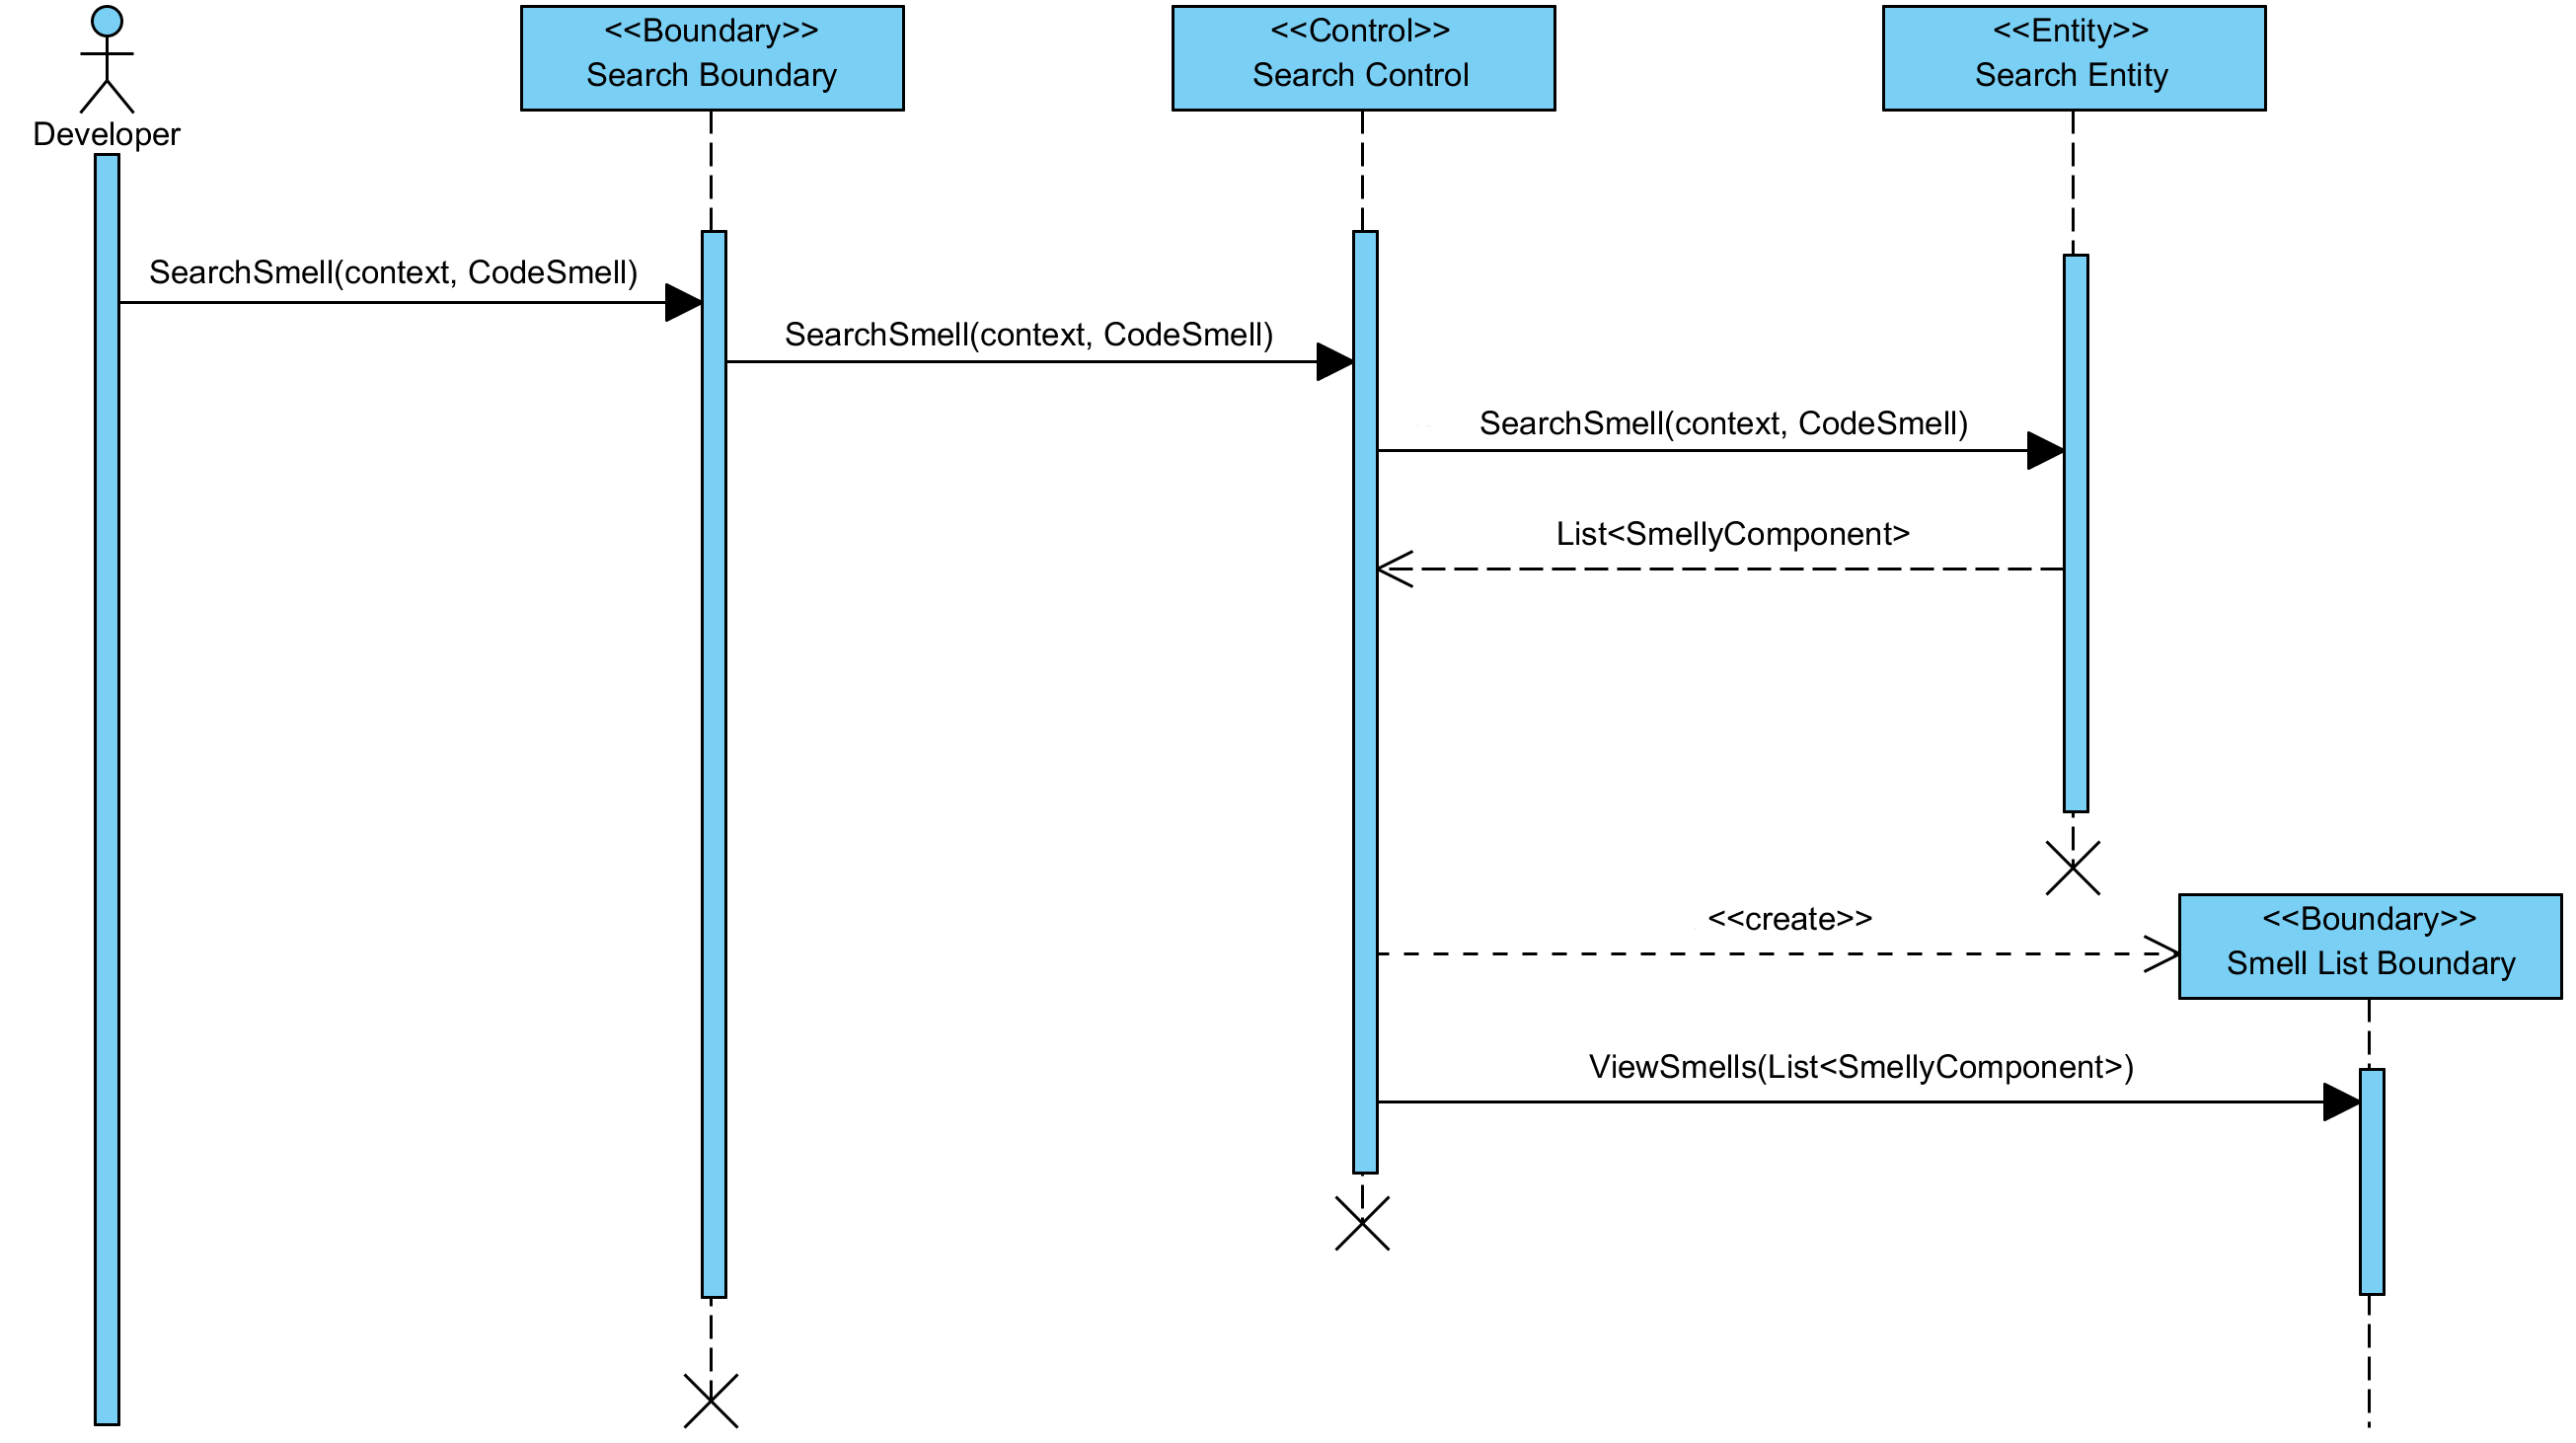
\includegraphics[width=\columnwidth]{AnalisiCurrentProposed.png}
					\caption{SD1-Analisi}
				\end{figure}
		
				\begin{figure}[h!]
					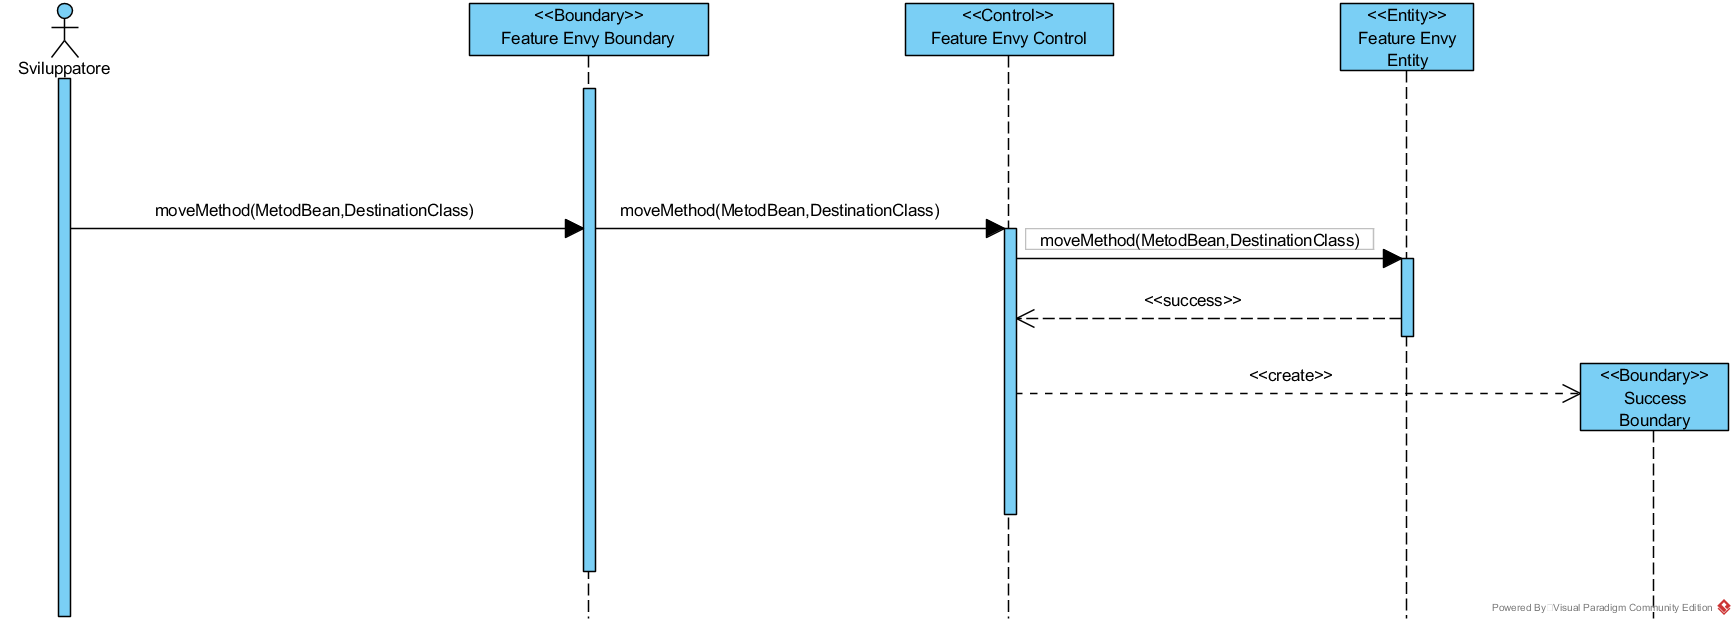
\includegraphics[width=\columnwidth]{Feature_Envy.png}
					\caption{SD2.1-Correzione Feature Envy}
				\end{figure}
			
				\begin{figure}[h!]
					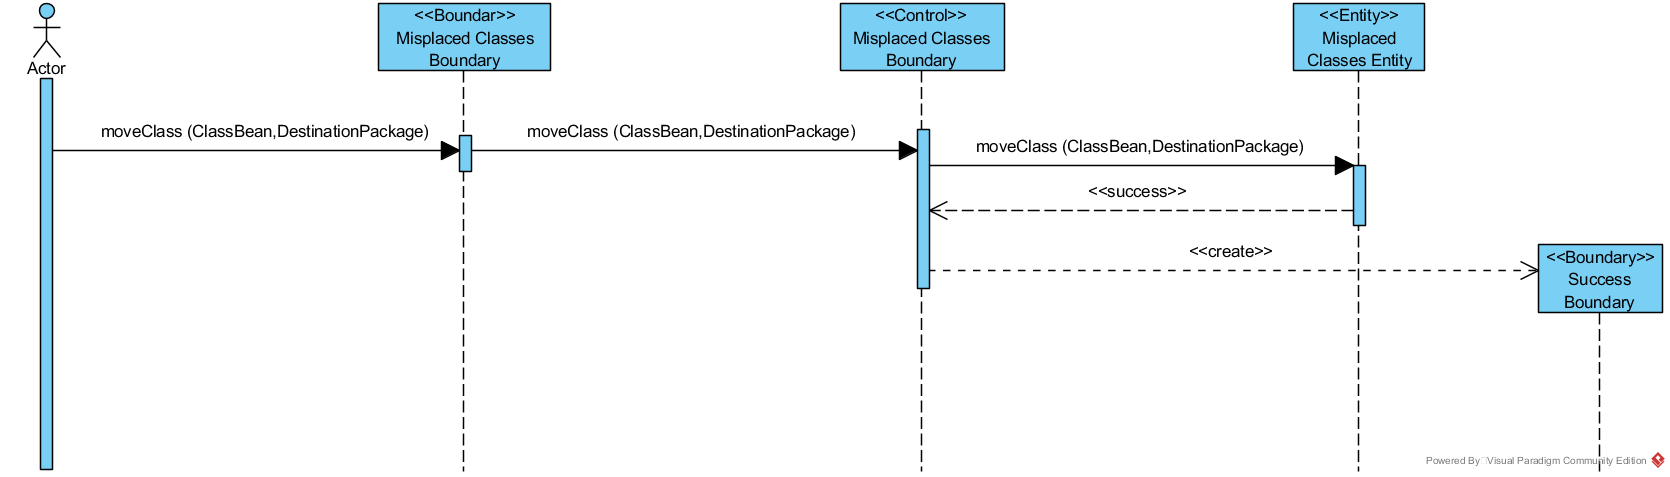
\includegraphics[width=\columnwidth]{SD_Misplaced_Classes.png}
					\caption{SD2.2-Correzione Misplaced Class}
				\end{figure}
			\newpage
			\subsubsection{Activity Diagram}
				\begin{figure}[h!]
					\centering
					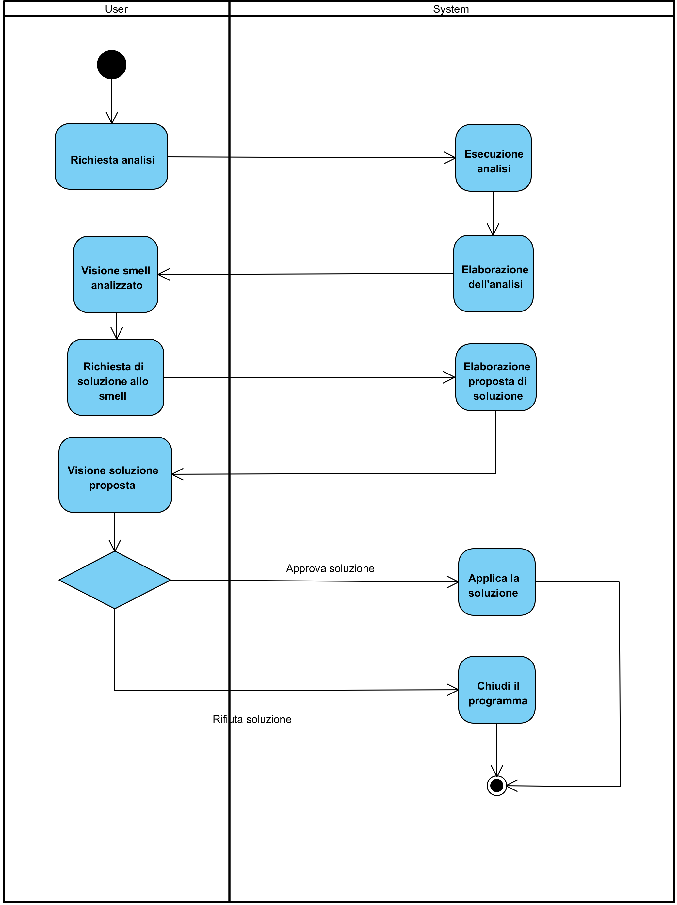
\includegraphics[scale=2]{ActivityDiagramCurrent.png}
					\caption{AD1-Analisi e Correzione}
				\end{figure}
		
	\newpage
	
	\section{Proposed system}
		
	    \begin{list}{-}{}
	\item{I seguenti requisiti funzionali, appartenenti al Current Envirorment, non sono stati modificati:}	
\end{list}
\begin{quote}	
	\begin{description}		
		\item[RF 1:]				
		\begin{list}{}{}
			\begin{quote}
				\item{RF 1.1}
			\end{quote}					
		\end{list}
		
		\item[RF 2:]				
		\begin{list}{}{}
			\begin{quote}
				\item{RF 2.1}
				\item{RF 2.2}		
			\end{quote}					
		\end{list}
		
		\item[RF 3:]				
		\begin{list}{}{}
			\begin{quote}
				\item{RF 3.1}
				\item{RF 3.2}		
			\end{quote}	
		\end{list}
		\item[RF 4:]	
		\begin{list}{}{}
			\begin{quote}
				\item{RF 4.1}
				\item{RF 4.2}		
			\end{quote}	
		\end{list}
		\item[RF 5]	
		\begin{list}{}{}
		\end{list}
		\item[RF 6]	
		\begin{list}{}{}
		\end{list}
		
	
	\end{description}
\end{quote}

\begin{list}{-}{}
	\item \textbf{RF 2 - Correzione} 
	\begin{quote}Il sistema consente la creazione di una possibile soluzione ai quattro principalei tipi di code smell.\end{quote}
	\begin{quote}
		\begin{description}    		 	
			\item [RF 2.3:]Il sistema fornisce una possibile soluzione al code smell di tipo Blob. 
			
				\begin{description}
					\item[RF 2.3.1:] Il sistema permette di modificare la possibile soluzione al Blob attraverso l'operazione che consente lo spostamento dei metodi applicata alle due classi proposte nell'operazione di "Extract class".		
				\end{description}
			
			\item[RF 2.4:] Il sistema fornisce una possibile soluzione al code smell di tipo Promiscuous Package.  
			
				\begin{description}
					\item[RF 2.4.1:] Il sistema permette di modificare la possibile soluzione al Promiscuous Package attraverso l'operazione di spostamento delle classi applicata ai package proposti nell'operazione di "Extract package".	
				\end{description}
			
			\item[RF 2.5:] Il sistema permette di segnalare come falso positivo una componente indicata come difettosa dal correttore automatico.
			
		\end{description}
	\end{quote}
	\item \textbf{RF 3 - Refactoring:} 
	\begin{quote}Il sistema consente la creazione di una possibile soluzione ai quattro principali tipi di code smell.\end{quote}
	\begin{quote}
		\begin{description}
			\item[RF 3.3:]Il sistema permette allo sviluppatore di risolvere il code smell di tipo Blob.
			
				\begin{description}
					\item[RF 3.3.1:]Il sistema permette di risolvere il code smell di tipo Blob attraverso l'uso dell'operazione di "Extract class".
					\newline		
				\end{description}
					
			\item[RF 3.4:]Il sistema permette allo sviluppatore di risolvere il code smell di tipo Promiscuous Package.
			
				\begin{description}
					\item[RF 3.4.1:]Il sistema permette di risolvere il code smell di tipo Promiscuous Package attraverso l'uso dell'operazione di "Extract package".
					\newline		
				\end{description}
			
		\end{description}
	\end{quote}
	\item \textbf{RF 7 - To Do:} 
	\begin{quote}
	\begin{description}
		\item[RF 7.1:]Il sistema consente, all'avvio del programma, di mostrare all'utente un promemoria per un'eventuale correzione manuale.
	\end{description}
	
		\begin{description}
			\item [RF 7.2: ]Il sistema consente di aggiungere un nuovo promemoria.
		\end{description}	
	\end{quote}
	
	\item	\textbf{RF 8 -  Statistiche di accoppiamento:}
	\newline Il sistema consente di visualizzare le statistiche riguardanti classi e package precedentemente analizzati.
	
	\item	\textbf{RF 9 - Numero modifiche e Revisioni:}
	\newline Il sistema permette di tener traccia del numero di volte che è stato modificato un componente.
	
	\item	\textbf{RF 10 - Analisi rischi:}
	\newline Il sistema consente di visualizzare una stima di pericolosità che potrebbe occorrere nel caso in cui si decide di fare un Refactor.
\end{list}		

\subsection{Requisiti Non Funzionali}
\begin{list}{-}{}
	
	\item \textbf{RNF 1 - Performance}
	\newline Il sistema deve garantire brevi tempi di risposta, in particolare nelle operazioni di analisi del codice.  
	\item \textbf{RNF 2 - Robustezza}
	\newline Il sistema è in grado di funzionare correttamente anche in situazioni anomale o in caso di uso scorretto, notificando l'utente della situazione erronea rilevata, ma senza terminare la propria esecuzione. 
	\item \textbf{RNF 3 - Sicurezza}
	\newline Il sistema si presenta sufficientemente sicuro in quanto il suo ambiente d'azione è locale, quindi non vi è la necessità di protezione da minacce esterne.
	\item \textbf{RNF 4 - Usabilità}
	\newline Il sistema risulta essere di facile utilizzo. L'interfaccia grafica risulta essere intuitiva, agevolando il lavoro dello sviluppatore. 
	\item \textbf{RNF 5 - Manutenibilità}
	\newline Il sistema presenta un elevato grado di manutenibilità, in particolare, favorisce l'aggiunta di nuove funzionalità.
	\item \textbf{RNF 6 - Implementazione}
	\newline Il sistema è realizzato interamente in linguaggio Java, sia parte back-end che front-end. 
	\item \textbf{RNF 7 - Affidabilità}
	\newline Il sistema assicura un'alta affidabilità, riducendo al minimo i casi di arresto anomalo del sistema.
\end{list}


	    
	    \subsection{Use Case Model}	
	    
	    \begin{figure}[h!]
	    	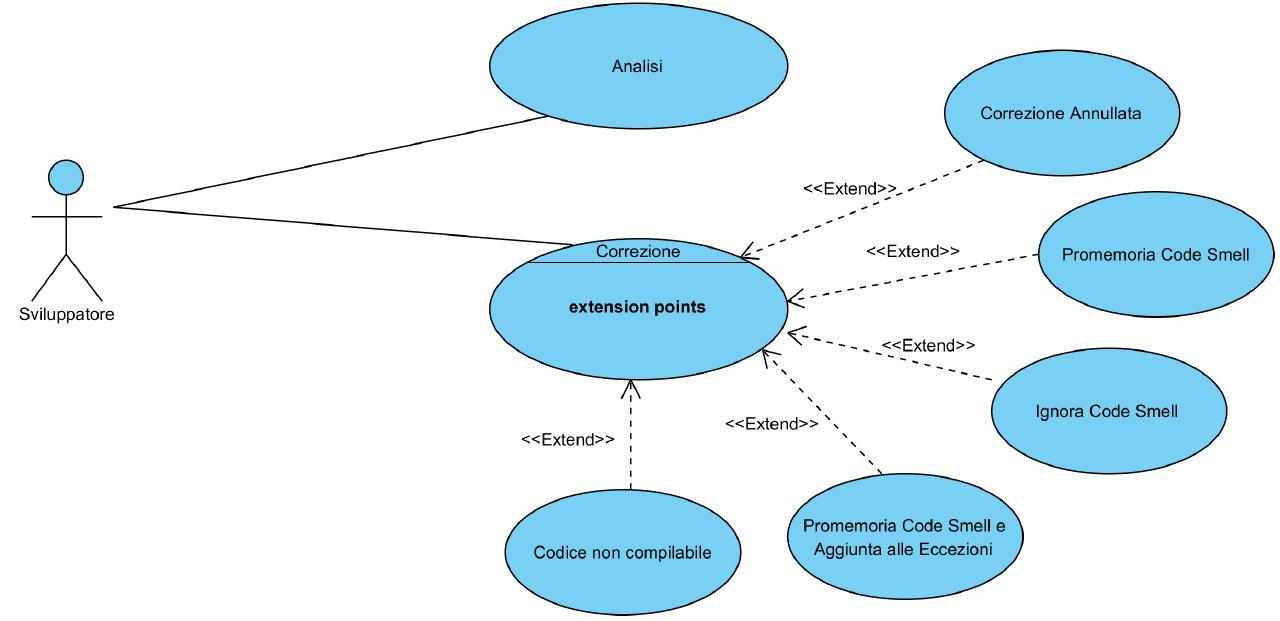
\includegraphics[width=\columnwidth]{UseCaseDiagramProposed.jpg}
	    	\caption{UCD1-Analisi e Correzione}
	    \end{figure}
    	
	    
		\begin{tabular}{|l|p{13cm}|}
			\hline
			\textbf{Use case name}  & \textbf{UC 1- Analisi e ricerca smell} \\ \hline
			\textbf{Participating actors}  & \textbf{Sviluppatore} \\ \hline
			\textbf{Entry condition}  & L'utente avvia con successo Intellij.\\  \hline
			\textbf{Flow of events}  &  
			\begin{tabular}{p{6cm}p{6cm}p{6cm}}
				\centering \textbf{UTENTE} & \centering \textbf{SISTEMA} & \\
				\textbf{1.}\hspace{0.3cm}L’utente nella sezione plugin di intelliJ,  sceglie di effettuare una ricerca  di “code smells” indicando il luogo e il tipo di "code smell", nel codice presente nel progetto aperto attualmente su intelliJ. La mancanza di parametri specificati, implica una ricerca globale su tutto il progetto. \\ \\ &
				\textbf{2.}\hspace{0.3cm}Il sistema, in base ai parametri specificati dall'utente, effettua una ricerca sul codice.
				Dopo una breve elaborazione, viene mostrata una finestra di riepilogo all’utente.
				In tale schermata sono presenti metriche, topic e una tabella che permette di filtrare i   risultati. \\ \\
				\textbf{3.}\hspace{0.3cm}L'utente prende visione del risultato dell'analisi tramite una tabella e varie RadarMap riportanti i 5 termini più frequenti. La tabella riporta per ogni smell identificato: una parte dedicata per effettuare refactoring o ignorare smell, la locazione,  le metriche di qualità calcolate(LOC, WNC, RFC, CBO, LCOM, NOA, NOM, NOPA, NOP) e il tipo di smell. Si può quindi selezionare l'elemento che si vuole esaminare e prendere visione del codice del progetto. \\ \\ &
				
			\end{tabular}\\ \hline
			
			\textbf{Exit condition}  &L’utente visualizza il codice affetto da smell\\ \hline
			\textbf{Exception condition}  & Nel passo 1, in caso di codice java non corretto dal punto di vista sintattico, semantico o lessicale si verifica lo UC 1.1. \\ \hline
			\textbf{Quality requirements}  & 
					\begin{itemize}
						\item Tempo di elaborazione massimo: 3 minuti.
						\item Il sistema è in grado di rilevare se il codice è java.
					\end{itemize}
			\\ \hline 
		\end{tabular}
	
	
		\begin{tabular}{|l|p{13cm}|}
			\hline
			\textbf{Use case name}  & \textbf{UC 1.1 - Analisi codice non compilabile} \\ \hline
			\textbf{Participating actors}  & \textbf{Sviluppatore} \\ \hline
			\textbf{Entry condition}  & L'utente avvia l'analisi del codice.\\ \hline 			
			\textbf{Flow of events}  & 
			\begin{tabular}{p{6cm}p{6cm}p{6cm}}
				\centering\textbf{UTENTE}  & \centering\textbf{SISTEMA} &\\ \\
				\textbf{1.}\hspace{0.3cm}L'utente attende l'elaborazioni richieste dal sistema.\\ 
				&\textbf{2.}\hspace{0.3cm}Il sistema tenta di analizzare il codice ma, trovando testo non compilabile, annulla l'operazione e mostra un messaggio di errore.\\
				\textbf{3.}\hspace{0.3cm}L'utente prende visione del messaggio che indica il fallimento dell'operazione. \\	\\		
			\end{tabular}\\ \hline		
			\textbf{Exit condition}  & Il sistema termina l'esecuzione senza effettuare alcuna modifica\\ \hline 			
			\textbf{Exception condition} & \\ \hline
			\textbf{Priority}  & Alta \\ \hline 	
			\textbf{Quality requirements}  & 
			\begin{itemize}
				\item Tempo di elaborazione massimo: 3 minuti.
			\end{itemize}
			
			\\ \hline 
		\end{tabular}
		
		\vspace{2cm}
		
		
		%USE CASE 2.1 - "CORREZIONE CODE SMELL SOLO FE"
		
		\begin{tabular}{|l|p{13cm}|}
			\hline
			\textbf{Use case name}  & \textbf{UC 2.1 - Correzione Code smell - Feature Envy} \\ \hline
			\textbf{Participating actors}  & \textbf{Sviluppatore} \\ \hline
			\textbf{Entry condition}  & L’utente ha visualizzato il codice affetto da smell  \\  \hline
			\textbf{Flow of events}  &  
			\begin{tabular}{p{6cm}p{6cm}p{6cm}}
				\centering \textbf{UTENTE} & \centering \textbf{SISTEMA} & \\
				\textbf{1.}\hspace{0.3cm}L’utente, dopo aver preso visione dei risultati dati del caso UC1.0 sceglie i parametri su cui intervenire per lo smells di tipo “Feature Envy” e avvia gli automatismi per la correzione automatica premendo il tasto “Refactor”.
				\\ \\ &
				\textbf{2.}\hspace{0.3cm}Il sistema, mostra una schermata di riepilogo con delle sezioni mostranti una proposta di correzione   confrontata con la situazione precedente all’analisi, e un tasto per apportare tali modifiche. \\ \\
				
				\textbf{3.}\hspace{0.3cm}L’utente, può scegliere di accettare tali modifiche consigliate dal sistema cliccando il tasto "Applica modifiche". Se lo sviluppatore non volesse correggere automaticamente il codice può   selezionare fra le   apposite voci di ignorare lo smell selezionato (Caso eccezione UC-2.5)   aggiungere un promemoria (caso eccezione UC-2.6) oppure entrambe (Caso eccezione   UC-2.7). L'utente sceglie di applicare la soluzione proposta dal sistema.
				\\ \\ &
				\textbf{4.}\hspace{0.3cm}Il sistema, applica la soluzione che precedentemente ha mostrato all'utente. \\ \\
				
				\textbf{5.}\hspace{0.3cm}L'utente prende visione di tutte le modifiche effettuate dal sistema. \\ \\
				
			\end{tabular}\\ \hline
			
			\textbf{Exit condition}  &La finestra del plug-in si chiude.\\ \hline
			\textbf{Exception condition}  & Se nel passo 3 l'utente non volesse correggere automaticamente il codice, può:
			\begin{itemize} \item Ignorare il code smell (UC- 2.5)
				\item Aggiungere un promemoria (UC-2.6)
				\item Promemoria code smell e aggiunta eccezioni (UC- 2.7) 
			\end{itemize}
			\\ \hline
			\textbf{Quality requirements}  & Tempo di elaborazione massimo: 3 minuti.
			\\ \hline 
		\end{tabular}
		
		%USE CASE 2.2 - "CORREZIONE CODE SMELL SOLO MC"
		
		\begin{tabular}{|l|p{13cm}|}
			\hline
			\textbf{Use case name}  & \textbf{UC 2.2 - Correzione Code smell - Misplaced Class} \\ \hline
			\textbf{Participating actors}  & \textbf{Sviluppatore} \\ \hline
			\textbf{Entry condition}  & L’utente ha visualizzato il codice affetto da smell  \\  \hline
			\textbf{Flow of events}  &  
			\begin{tabular}{p{6cm}p{6cm}p{6cm}}
				\centering \textbf{UTENTE} & \centering \textbf{SISTEMA} & \\
				\textbf{1.}\hspace{0.3cm}L’utente, dopo aver preso visione dei risultati dati del caso UC1.0 sceglie i parametri su cui intervenire per lo smells di tipo “Misplaced Class” e avvia gli automatismi per la correzione automatica premendo il tasto “Refactor”.
				\\ \\ &
				\textbf{2.}\hspace{0.3cm}Il sistema, mostra una schermata di riepilogo con delle sezioni mostranti una proposta di correzione   confrontata con la situazione precedente all’analisi, e un tasto per apportare tali modifiche. \\ \\
				
				\textbf{3.}\hspace{0.3cm}L’utente, può scegliere di accettare tali modifiche consigliate dal sistema cliccando il tasto "Applica modifiche". Se lo sviluppatore non volesse correggere automaticamente il codice può   selezionare fra le   apposite voci di ignorare lo smell selezionato (Caso eccezione UC-2.5)   aggiungere un promemoria (caso eccezione UC-2.6) oppure entrambe (Caso eccezione   UC-2.7). L'utente sceglie di applicare la soluzione proposta dal sistema.
				\\ \\ &
				\textbf{4.}\hspace{0.3cm}Il sistema, applica la soluzione che precedentemente ha mostrato all'utente. \\ \\
				
				\textbf{5.}\hspace{0.3cm}L'utente prende visione di tutte le modifiche effettuate dal sistema. \\ \\
				
			\end{tabular}\\ \hline
			
			\textbf{Exit condition}  &La finestra del plug-in si chiude.\\ \hline
			\textbf{Exception condition}  & Se nel passo 3 l'utente non volesse correggere automaticamente il codice, può:
			\begin{itemize} \item Ignorare il code smell (UC- 2.5)
				\item Aggiungere un promemoria (UC-2.6)
				\item Promemoria code smell e aggiunta eccezioni (UC- 2.7) 
			\end{itemize}
			\\ \hline
			\textbf{Quality requirements}  & Tempo di elaborazione massimo: 3 minuti.
			\\ \hline 
		\end{tabular}
		
		
		\vspace{2cm}
		%USE CASE 2.3 - "CORREZIONE CODE SMELL BLOB"
		
		\begin{tabular}{|l|p{13cm}|}
			\hline
			\textbf{Use case name}  & \textbf{UC 2.3 - Correzione Code smell - Blob} \\ \hline
			\textbf{Participating actors}  & \textbf{Sviluppatore} \\ \hline
			\textbf{Entry condition}  & L’utente ha visualizzato il codice affetto da smell  \\  \hline
			\textbf{Flow of events}  &  
			\begin{tabular}{p{6cm}p{6cm}p{6cm}}
				\centering \textbf{UTENTE} & \centering \textbf{SISTEMA} & \\
				\textbf{1.}\hspace{0.3cm}L’utente, dopo aver preso visione dei risultati dati del caso UC1.0 seleziona “Blob” come parametro su cui intervenire.
				\\ \\ &
				\textbf{2.}\hspace{0.3cm}Il sistema, mostra una nuova schermata di riepilogo con delle sezioni mostranti delle frecce per scegliere come “estrarre” gli smells e dei grafici riguardanti un confronto tra la situazione precedente all’analisi e un tasto per apportare tali modifiche. \\ \\
				
				\textbf{3.}\hspace{0.3cm}L'utente puo' selezionare come e dove estrarre gli smells tramite un interfaccia guidata, al termine di tale selezione, clicca sul tasto “applica” per apportare le modifiche oppure, se lo sviluppatore non volesse correggere il codice può selezionare fra le apposite voci di ignorare lo smell selezionato (Caso eccezione UC-2.5) aggiungere un promemoria (caso eccezione UC-2.6) oppure entrambe (Caso eccezione   UC-2.7). L'utente sceglie di applicare la soluzione proposta dal sistema.
				\\ \\ &
				\textbf{4.}\hspace{0.3cm}Il sistema, applica la soluzione che precedentemente ha mostrato all'utente. \\ \\
				
				\textbf{5.}\hspace{0.3cm}L'utente prende visione di tutte le modifiche effettuate dal sistema. \\ \\
				
			\end{tabular}\\ \hline
			
			\textbf{Exit condition}  &La finestra del plug-in si chiude.\\ \hline
			\textbf{Exception condition}  & Se nel passo 3 l'utente non volesse correggere automaticamente il codice, può:
			\begin{itemize} \item Ignorare il code smell (UC- 2.5)
				\item Aggiungere un promemoria (UC-2.6)
				\item Promemoria code smell e aggiunta eccezioni (UC- 2.7) 
			\end{itemize}
			\\ \hline
			\textbf{Quality requirements}  & Tempo di elaborazione massimo: 3 minuti.
			\\ \hline 
		\end{tabular}
		
		
		\vspace{2cm}
		%USE CASE 2.2 - "CORREZIONE CODE SMELL SOLO Blob"
		
		\begin{tabular}{|l|p{13cm}|}
			\hline
			\textbf{Use case name}  & \textbf{UC 2.4 - Correzione Code smell - Promiscuous Package} \\ \hline
			\textbf{Participating actors}  & \textbf{Sviluppatore} \\ \hline
			\textbf{Entry condition}  & L’utente ha visualizzato il codice affetto da smell  \\  \hline
			\textbf{Flow of events}  &  
			\begin{tabular}{p{6cm}p{6cm}p{6cm}}
				\centering \textbf{UTENTE} & \centering \textbf{SISTEMA} & \\
				\textbf{1.}\hspace{0.3cm}L’utente, dopo aver preso visione dei risultati dati del caso UC1.0 seleziona “Promiscuous Package” come parametro su cui intervenire.
				\\ \\ &
				\textbf{2.}\hspace{0.3cm}Il sistema, mostra una nuova schermata di riepilogo con delle sezioni mostranti delle frecce per scegliere come “estrarre” gli smells e dei grafici riguardanti un confronto tra la situazione precedente all’analisi e un tasto per apportare tali modifiche. \\ \\
				
				\textbf{3.}\hspace{0.3cm}L'utente puo' selezionare come e dove estrarre gli smells tramite un interfaccia guidata, al termine di tale selezione, clicca sul tasto “applica” per apportare le modifiche oppure, se lo sviluppatore non volesse correggere il codice può selezionare fra le apposite voci di ignorare lo smell selezionato (Caso eccezione UC-2.5) aggiungere un promemoria (caso eccezione UC-2.6) oppure entrambe (Caso eccezione   UC-2.7). L'utente sceglie di applicare la soluzione proposta dal sistema.
				\\ \\ & 
				\textbf{4.}\hspace{0.3cm}Il sistema, applica la soluzione che precedentemente ha mostrato all'utente. \\ \\
				
				\textbf{5.}\hspace{0.3cm}L'utente prende visione di tutte le modifiche effettuate dal sistema. \\ \\
				
			\end{tabular}\\ \hline
			
			\textbf{Exit condition}  &La finestra del plug-in si chiude.\\ \hline
			\textbf{Exception condition}  & Se nel passo 3 l'utente non volesse correggere automaticamente il codice, può:
			\begin{itemize} \item Ignorare il code smell (UC- 2.5)
				\item Aggiungere un promemoria (UC-2.6)
				\item Promemoria code smell e aggiunta eccezioni (UC- 2.7) 
			\end{itemize}
			\\ \hline
			\textbf{Quality requirements}  & Tempo di elaborazione massimo: 3 minuti.
			\\ \hline 
		\end{tabular}		
		
		\vspace{2cm}
		%USE CASE 2.1 - "IGNORA CODE SMELL"
		\begin{tabular}{|l|p{13cm}|}
			\hline
			\textbf{Use case name}  & \textbf{UC 2.5- Ignora code smell} \\ \hline
			\textbf{Participating actors}  & \textbf{Sviluppatore} \\ \hline
			\textbf{Entry condition}  & L'utente ha deciso di ignorare il code smell  \\  \hline
			\textbf{Flow of events}  &  
			\begin{tabular}{p{6cm}p{6cm}p{6cm}}
				\centering \textbf{UTENTE} & \centering \textbf{SISTEMA} & \\
				
				\textbf{1.}\hspace{0.3cm}L’utente, dopo aver preso visione dei risultati dati del caso UC1.0 sceglie i parametri ed individua gli smells che vuole aggiungere ad un elenco di risultati da ignorare ( che siano essi falsi positivi o rigettati per scelta del programmatore)  \\ \\ &
				
				\textbf{2.}\hspace{0.3cm}Il sistema dopo l’aggiunta alla “lista da ignorare” non mostrerà più i casi da ignorare tra i risultati di analisi a meno di modifiche al codice manuali, nel qual caso verrano eliminati da quest’elenco nella analisi successiva. Il sistema, applica le modifiche scelte dall'utente. \\ \\
				
				\textbf{3.}\hspace{0.3cm}L'utente prende visione della "lista da ignorare" contente tutti gli smell scelti. \\ \\
				
			\end{tabular}\\ \hline
			
			\textbf{Exit condition}  &La finestra del plug-in si chiude\\ \hline
			\textbf{Exception condition}  & \\ \hline
			\textbf{Quality requirements}  & Tempo di elaborazione massimo: 1 minuto.
			\\ \hline 
		\end{tabular}
		
		\vspace{"2cm}
		
		% USE CASE 2.2 -  "PROMEMORIA CODE SMELL" 
		\begin{tabular}{|l|p{13cm}|}
			\hline
			\textbf{Use case name}  & \textbf{UC 2.6- Promemoria code smell} \\ \hline
			\textbf{Participating actors}  & \textbf{Sviluppatore} \\ \hline
			\textbf{Entry condition}  & L'utente ha deciso di avere un promemoria dello smell \\  \hline
			\textbf{Flow of events}  &  
			\begin{tabular}{p{6cm}p{6cm}p{6cm}}
				\centering \textbf{UTENTE} & \centering \textbf{SISTEMA} & \\
				\textbf{1.}\hspace{0.3cm}L’utente dopo l’analisi del caso UC 1.0, seleziona i propri parametri e seleziona la voce  “aggiungi promemoria”  \\ \\ &
				\textbf{2.}\hspace{0.3cm}Il sistema aggiunge la parte di codice al “To do list” di intelliJ, ovvero aggiunge dei piccoli promemoria che compariranno in una finestra dedicata con la funzione di ricordare allo sviluppatore in quale parte del code deve effettuare delle correzioni. \\ \\
				\textbf{3.}\hspace{0.3cm}L’utente prende visione delle modifiche effettuate dal sistema.  \\ \\ 
				
			\end{tabular}\\ \hline
			
			\textbf{Exit condition}  & La finestra del plug-in si chiude\\ \hline
			\textbf{Exception condition}  & \\ \hline
			\textbf{Quality requirements}  & Tempo di elaborazione massimo: 1 minuto.
			\\ \hline 
		\end{tabular}
		
		
		\vspace{2cm}
		
		%USE CASE 2.3- "PROMEMORIA CODE SMELL E AGGIUNTA ECCEZIONI"
		
		\begin{tabular}{|l|p{13cm}|}
			\hline
			\textbf{Use case name}  & \textbf{UC 2.7- Promemoria code smell e aggiunta alle eccezioni} \\ \hline
			\textbf{Participating actors}  & \textbf{Sviluppatore} \\ \hline
			\textbf{Entry condition}  & L'utente sceglie il promemoria e aggiunta eccezioni  \\  \hline
			\textbf{Flow of events}  &  
			\begin{tabular}{p{6cm}p{6cm}p{6cm}}
				\centering \textbf{UTENTE} & \centering \textbf{SISTEMA} & \\
				\textbf{1.}\hspace{0.3cm}L'utente, dopo aver preso visione dei risultati dati del caso UC1.0 sceglie i parametri ed individua gli smells che vuole aggiungere ad un elenco di risultati da ignorare ( che siano essi falsi positivi o rigettati per scelta del programmatore) e seleziona, inoltre,  la voce “aggiungi promemoria”  \\ \\ &
				\textbf{2.}\hspace{0.3cm}Il sistema  dopo l’aggiunta alla “lista da ignorare” non mostrerà più i casi da ignorare ma aggiunge le parti di codice al “To do list” di intelliJ \\ \\
				
				\textbf{3.}\hspace{0.3cm}L'utente prende visione delle modifiche effettuate dal sistema. \\ \\
				
			\end{tabular}\\ \hline
			
			\textbf{Exit condition}  &La finestra del plug-in si chiude\\ \hline
			\textbf{Exception condition}  & \\ \hline
			\textbf{Quality requirements}  & Tempo di elaborazione massimo: 1 minuto
			\\ \hline 
		\end{tabular}
	    \vspace{1cm}
	    	\newpage
		\begin{tabular}{|l|p{13cm}|}
			\hline
			\textbf{ID}  & \textbf{UC 2.8} \\ \hline
			\textbf{Nome caso d'uso}  & Statistiche classe/package \\ \hline
			\textbf{Attori partecipanti}  & Sviluppatore \\ \hline
			\textbf{Precondizione}  & UC 1.0 \\ \hline
			\textbf{Flusso di eventi}  & 
			\begin{tabular}{p{6cm}p{6cm}}
				Utente & Sistema  \\
				Dopo l'analisi (UC 1) lo sviluppatore si trova davanti ad una schermata di riepilogo nella quale una volta selezionata una voce tra i risultati proposti, è presente il tasto "Statistiche e Correlazioni" che rimanda ad una nuova finestra.\\
				& il sistema genera una nuova finestra contenente un elenco di \textbf{Associazioni}, \textbf{Aggregazioni}, \textbf{Composizioni} e \textbf{Specializzazioni} che riguardano la classe/package che abbiamo selezionato precedentemente
				\\
				Lo sviluppatore prende visione dei risultati generati dal sistema ed effettua le proprie valutazioni, al termine delle quali chiude semplicemente la finestra e torna alla schermata precedente.
			\end{tabular}\\ \hline
			\textbf{Condizione d'uscita} & L'utente visualizza correttamente le statistiche\\ \hline
			\textbf{Eccezioni}  & \\ \hline
			\textbf{Priorità} & Bassa \\ \hline
			\textbf{Requisiti di qualità}  & \\ \hline 
		\end{tabular}
	
	\newpage
	
	\begin{tabular}{|l|p{13cm}|}
		\hline
		\textbf{ID}  & \textbf{UC 2.9} \\ \hline
		\textbf{Nome caso d'uso}  & Numero di modifiche e revisioni \\ \hline
		\textbf{Attori partecipanti}  & Sviluppatore \\ \hline
		\textbf{Precondizione}  & UC 1.0 \\ \hline
		\textbf{Flusso di eventi}  & 
		\begin{tabular}{p{6cm}p{6cm}}
		 \textbf{Utente} & \textbf{Sistema}  \\
			Dopo l'analisi (UC 1) lo sviluppatore si trova davanti ad una schermata di riepilogo nella quale una volta selezionata una voce tra i risultati proposti, è presente il tasto "Numero di modifiche e revisioni" che rimanda ad una nuova finestra.\\
			& il sistema genera una nuova finestra contenente il numero di modifiche effettuate alla classe/package in esame.
			\\
			Lo sviluppatore prende visione dei risultati generati dal sistema ed effettua le proprie valutazioni, al termine delle quali chiude semplicemente la finestra e torna alla schermata precedente.
		\end{tabular}\\ \hline
		\textbf{Condizione d'uscita}  & L'utente visualizza correttamente le statistiche\\ \hline
		\textbf{Eccezioni}  & \\ \hline
		\textbf{Priorità} & Bassa \\ \hline
		\textbf{Requisiti di qualità}  & \\ \hline 
	\end{tabular}

	\newpage

	\begin{tabular}{|l|p{13cm}|}
		\hline
		\textbf{ID}  & \textbf{UC 2.10} \\ \hline
		\textbf{Nome caso d'uso}  & Analisi Rischi \\ \hline
		\textbf{Attori partecipanti}  & Sviluppatore \\ \hline
		\textbf{Precondizione}  & UC 1.0 \\ \hline
		\textbf{Flusso di eventi}  & 
		\begin{tabular}{p{6cm}p{6cm}}
			Utente & Sistema  \\
			Dopo l'analisi (UC 1) lo sviluppatore si trova davanti ad una schermata di riepilogo nella quale una volta selezionata una voce tra i risultati proposti, è presente il tasto "Stima rischi modifica" che rimanda ad una nuova finestra.\\
			& il sistema genera una nuova finestra contenente una stima di "pericolosità di modifica" basata sulle correlazioni tra classi e il numero di modifiche già effettuate alla classe/package in esame
			\\
			Lo sviluppatore prende visione dei risultati generati dal sistema ed effettua le proprie valutazioni, al termine delle quali chiude semplicemente la finestra e torna alla schermata precedente.
		\end{tabular}\\ \hline
		\textbf{Condizione d'uscita}  & L'utente visualizza correttamente le statistiche \\ \hline
		\textbf{Eccezioni}  & \\ \hline
		\textbf{Priorità} & Bassa \\ \hline
		\textbf{Requisiti di qualità}  & \\ \hline 
	\end{tabular}
	    
	    
	    \subsection{Static Analysis Model}
	    
	    		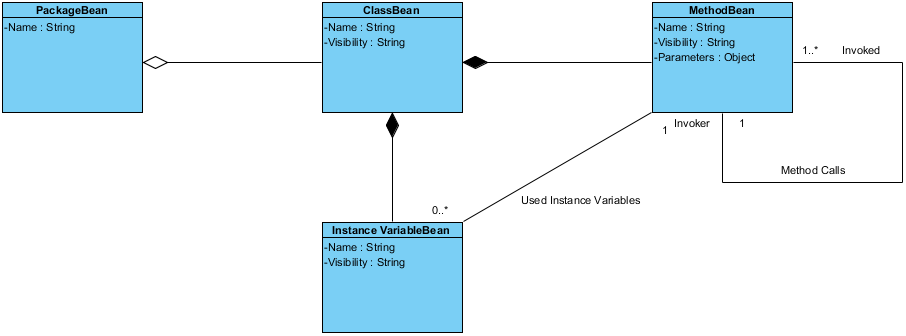
\includegraphics[width=\columnwidth]{classDiagram.png}
	    	
	    		\begin{tabular}{|l|p{3.5cm}|p{11cm}|}
	
	\hline \textbf{TIPO} & \textbf{NOME} & \textbf{DESCRIZIONE} \\ \hline
	Boundary & Search & Boundary che si occupa della riproduzione a schermo dei risultati dell'analisi. \\ 
	& Smell List & Boundary che si occupa della visualizzazione della lista degli smell trovati in fase di analisi. \\
	& Proposed Solution & Boundary che rende possibile visualizzare la lista delle soluzioni elaborate dal sistema. \\ 
	& Result & Boundary che rende possibile visualizzare i risultati dopo l'esecuzione del Refactor. \\
	& Smell Manager & Boundary che consente la visualizzazione dei Code Smell trovati in fase d'analisi, dal quale è possibile scegliere le operazioni da effettuare su questi ultimi. \\
	& Success & Boundary preposto alla visualizzazione dei messaggi di successo delle avvenute operazioni. \\
	& Statistics & Boundary che si occupa della visualizzazione dei dati relativi alle statistiche calcolate sui Code Smell. \\ 
	& Statistics Summary & Boundary che si occupa della visualizzazione a schermo delle statistiche aggiornate calcolate sui Code Smell. \\ 
	& Revision & Boundary che consente di visualizzare i dati relativi al numero di modifiche e revisioni effettuate su determinati Code Smell. \\ 
	& Revision Summary & Boundary che rende possibile visualizzare le statistiche aggiornate relative a revisioni e modifiche effettuate su determinati Smell. \\
	& Risk Analysis & Boundary che consente di visualizzare i fattori di rischio legati alla modifica di una classe. \\ 
	& Risk Result & Boundary preposto alla visualizzazione dei dati relativi ai fattori di rischio aggiornati. \\ \hline
	Control & Search & Control che invia messaggi al Search Entity per ricercare smell ed istanzia lo Smell List Boundary, al quale invia un messaggio per richiedere la visualizzazione della lista degli smell.\\ 
	& Proposed Solution & Control che crea il Solution Boundary, al quale invia un messaggio per visualizzare le proposte di correzione. \\
	& Refactoring & Control che crea il Result Boundary, al quale invia un messaggio per notificare il successo dell'operazione di Refactoring. \\
	& Corrector & Control che comunica con lo Smell Mangaer entity, al quale invia un messaggio per procedere con la correzione dello smell, dopodiché istanzia il Success Boundary. \\ 
	& Ignore & Control che si occupa di comunicare allo Smell Manager Entity un messaggio per far sì che un determinato Code Smell, selezionato precedentemente, venga ignorato. \\ 
	& Reminder & Control che comunica con lo Smell Manager Entity e invia un messaggio per porre un Code Smell in "to do". \\ 
	& Statistics & Control che crea lo Statistics Summary Boundary e comunica con lo Statistics Entity, al quale invia un messaggio per ottenere i dati sulle statistiche calcolate sui Code Smell. \\
	& Revision & Control che comunica con il Revision Entity, al quale invia un messaggio per ottenere i dati relativi alle modifiche effettuate, dopodiché istanzia il Revision Summary Boundary. \\ 
	& Risk Analysis & Control che comunica con il Risk Analysis Entity, al quale invia un messaggio per ottenere i dati sui fattori di rischio calcolati per la modifica di una classe, successivamente istanzia il Risk Result Boundary. \\ \hline 
	Entity & Search & Entity che conserva i dati persistenti relativi ai Code Smell trovati in fase di analisi. \\ 
	& Smell Manager & Entity che conserva i dati relativi alle correzioni effettuate sui Code Smell. \\ 
	& Statistics & Entity che conserva i dati relativi alle statistiche calcolate sui Code Smell. \\ 
	& Revision & Entity che conserva i dati relativi alle modifiche e revisioni effettuate sui Code Smell. \\ \hline
	
\end{tabular}
	    		
	    		\vspace{0.5cm}
				
				Gli oggetti presenti nella tabella soprastante sono stati individuati a seguito dell'analisi dinamica sotto riportata. 
				    		
	    		\vspace{0.5cm}
	    \subsection{Dynamic Analysis Model}
	    
	    	
	    	
    	\subsubsection{Sequence Diagram}
    	
    		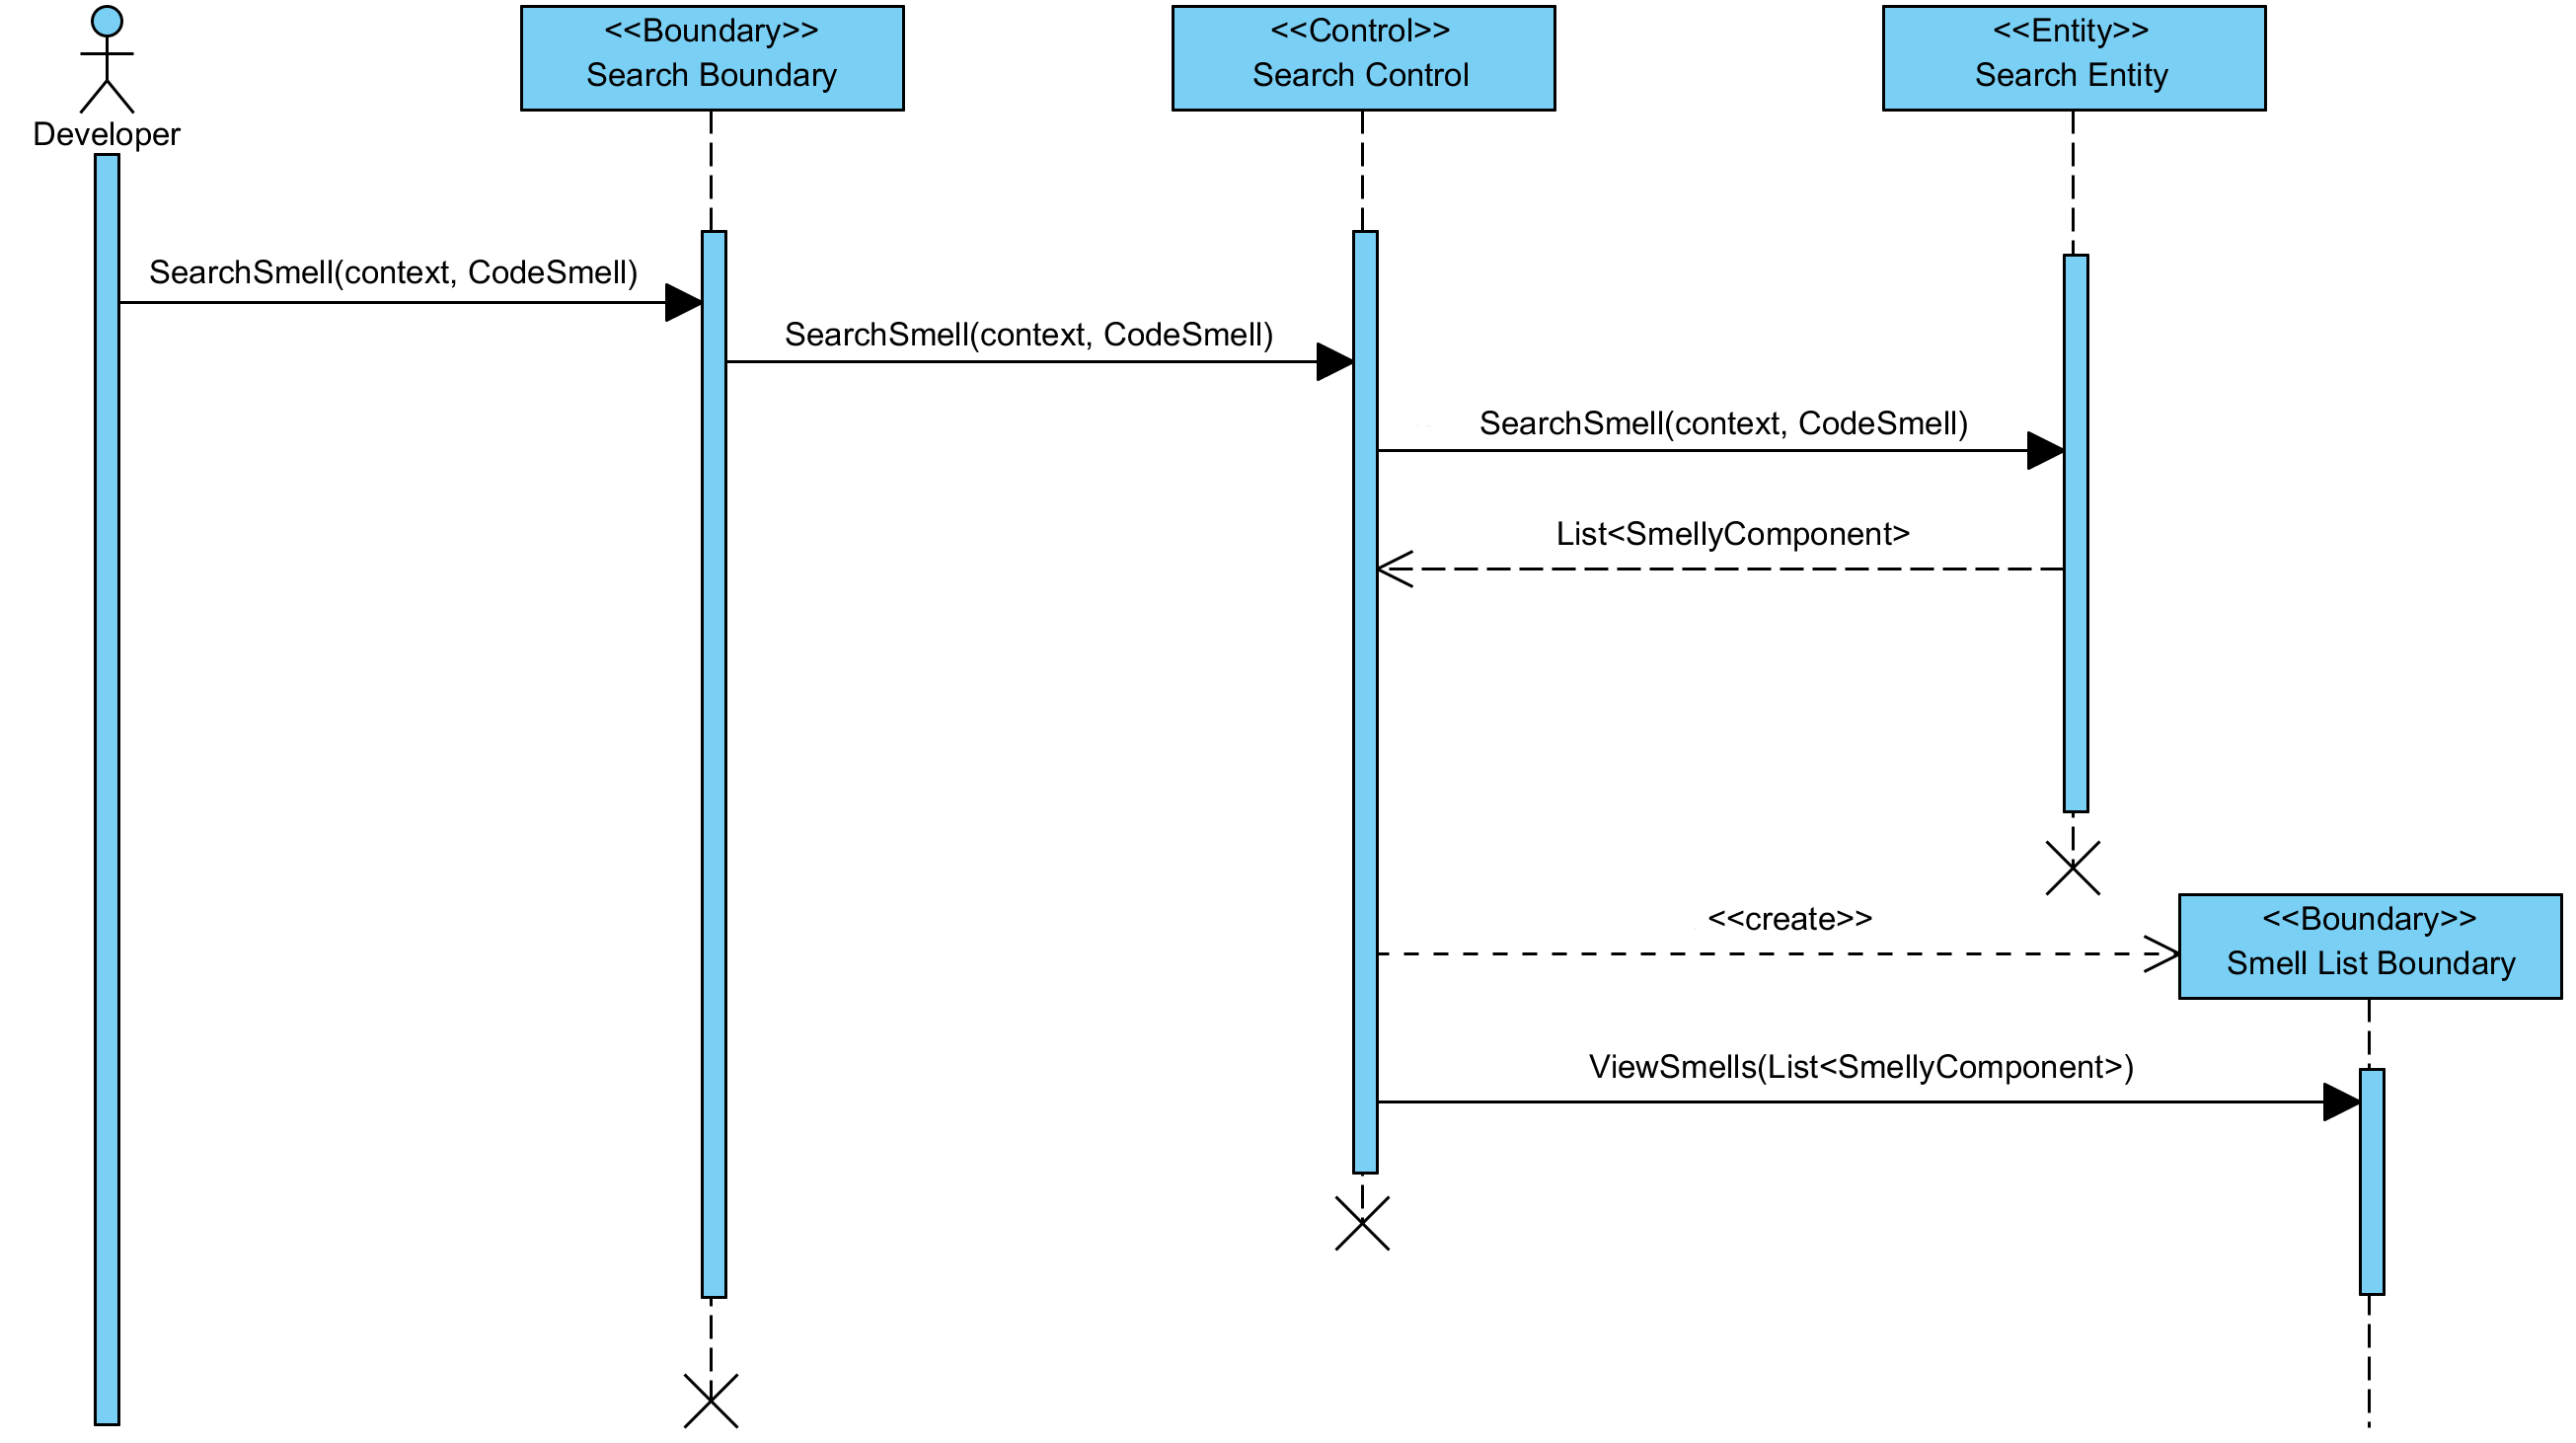
\includegraphics[width=\columnwidth]{AnalisiCurrentProposed.png}
    		\centering{SD1-Analisi e ricerca smell}
    	    		    	
    		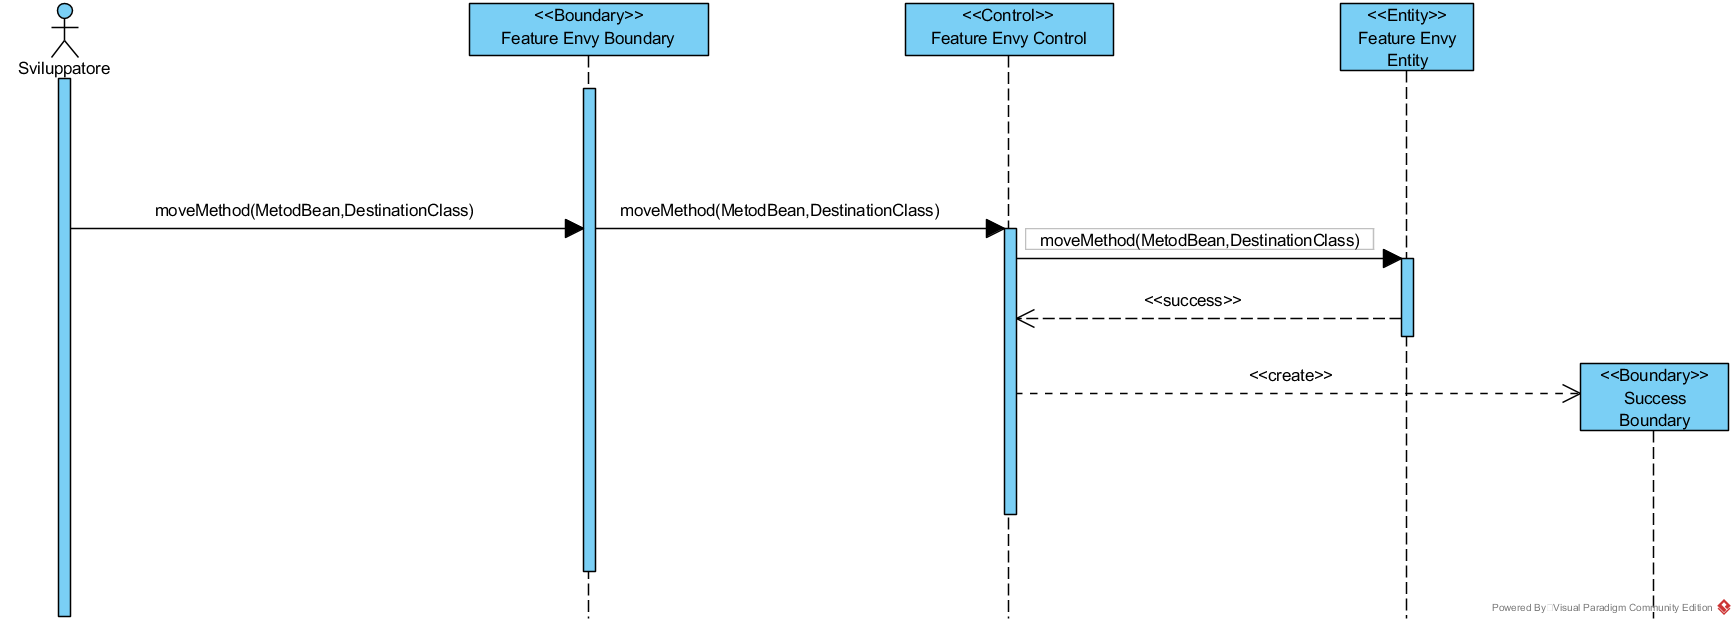
\includegraphics[width=\columnwidth]{Feature_Envy.png}
    		\centering{SD2.1-Correzione Code smell "Feature Envy"}
    		
    		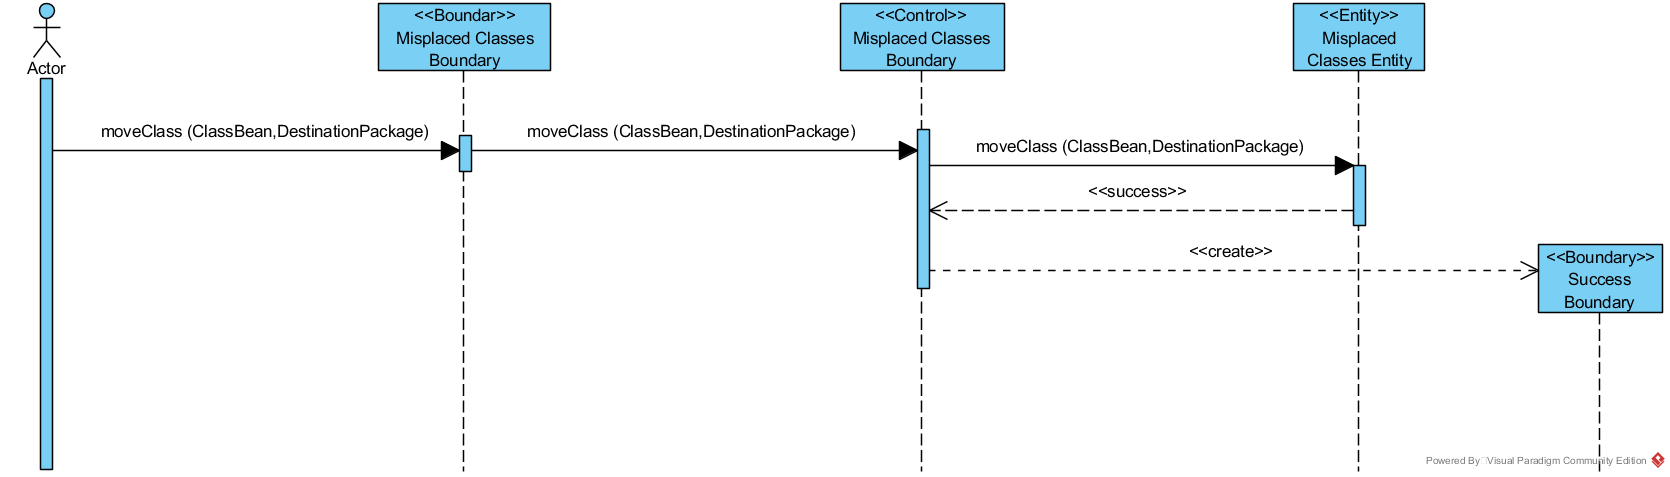
\includegraphics[width=\columnwidth]{SD_Misplaced_Classes.png}
    		\centering{SD2.2-Correzione Code smell "Misplaced Class"}
    	
    		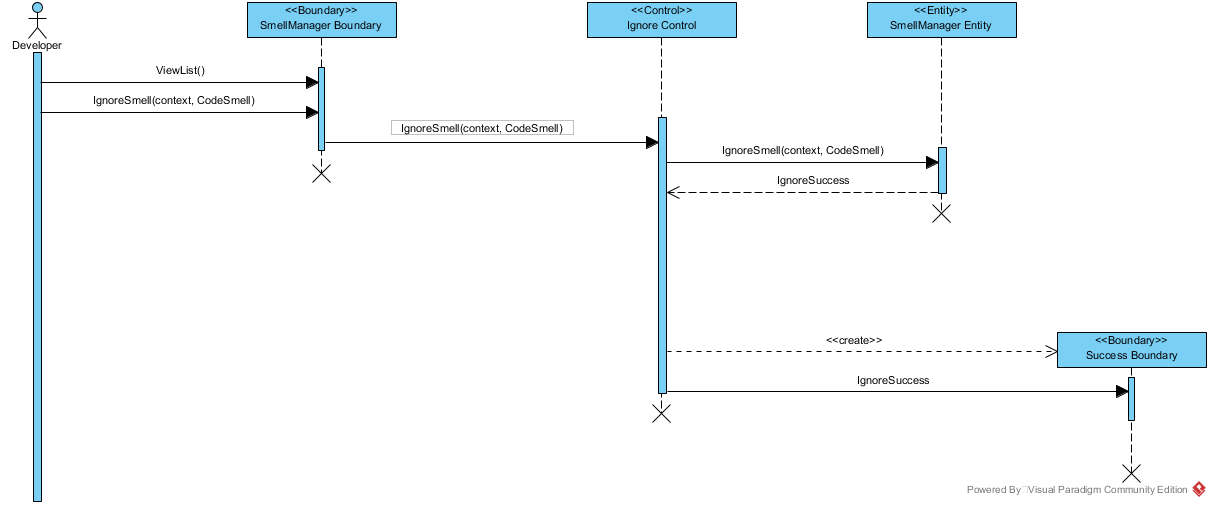
\includegraphics[width=\columnwidth]{Ignore.png}
    		\centering{SD2.5-Ignora code smell}
    	
    		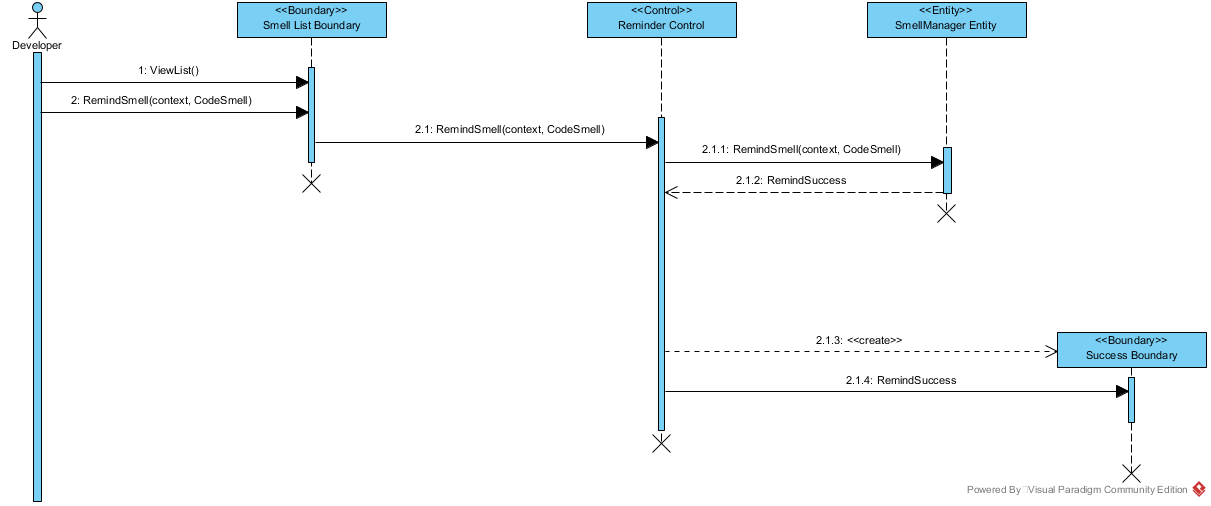
\includegraphics[width=\columnwidth]{Reminder.png}
    		\centering{SD2.6-Promemoria code smell}
    	
    		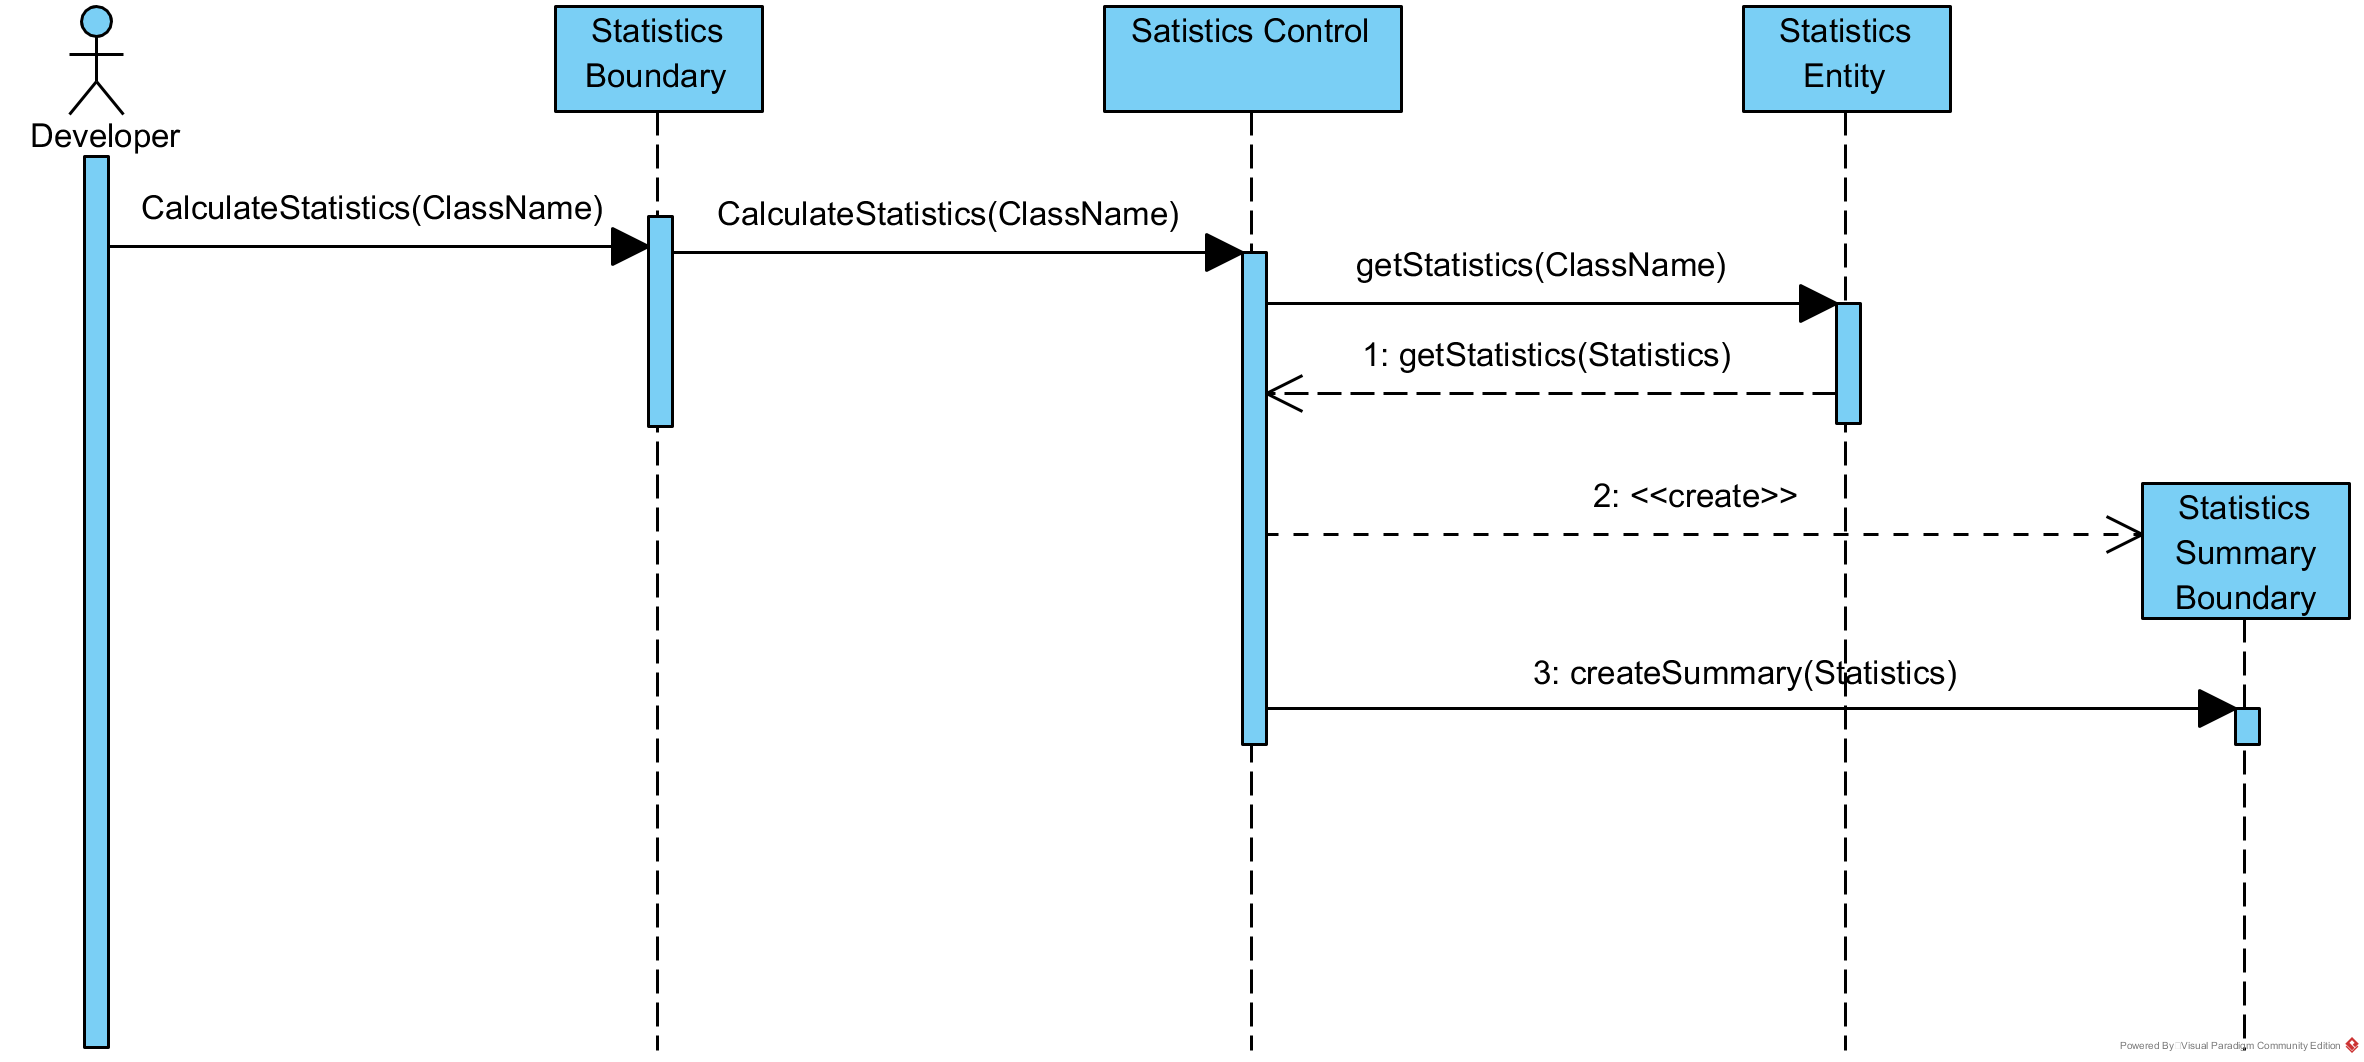
\includegraphics[width=\columnwidth]{LP_Statistics.png}
    		\centering{SD2.7-Statistiche classe/package}
    	
    		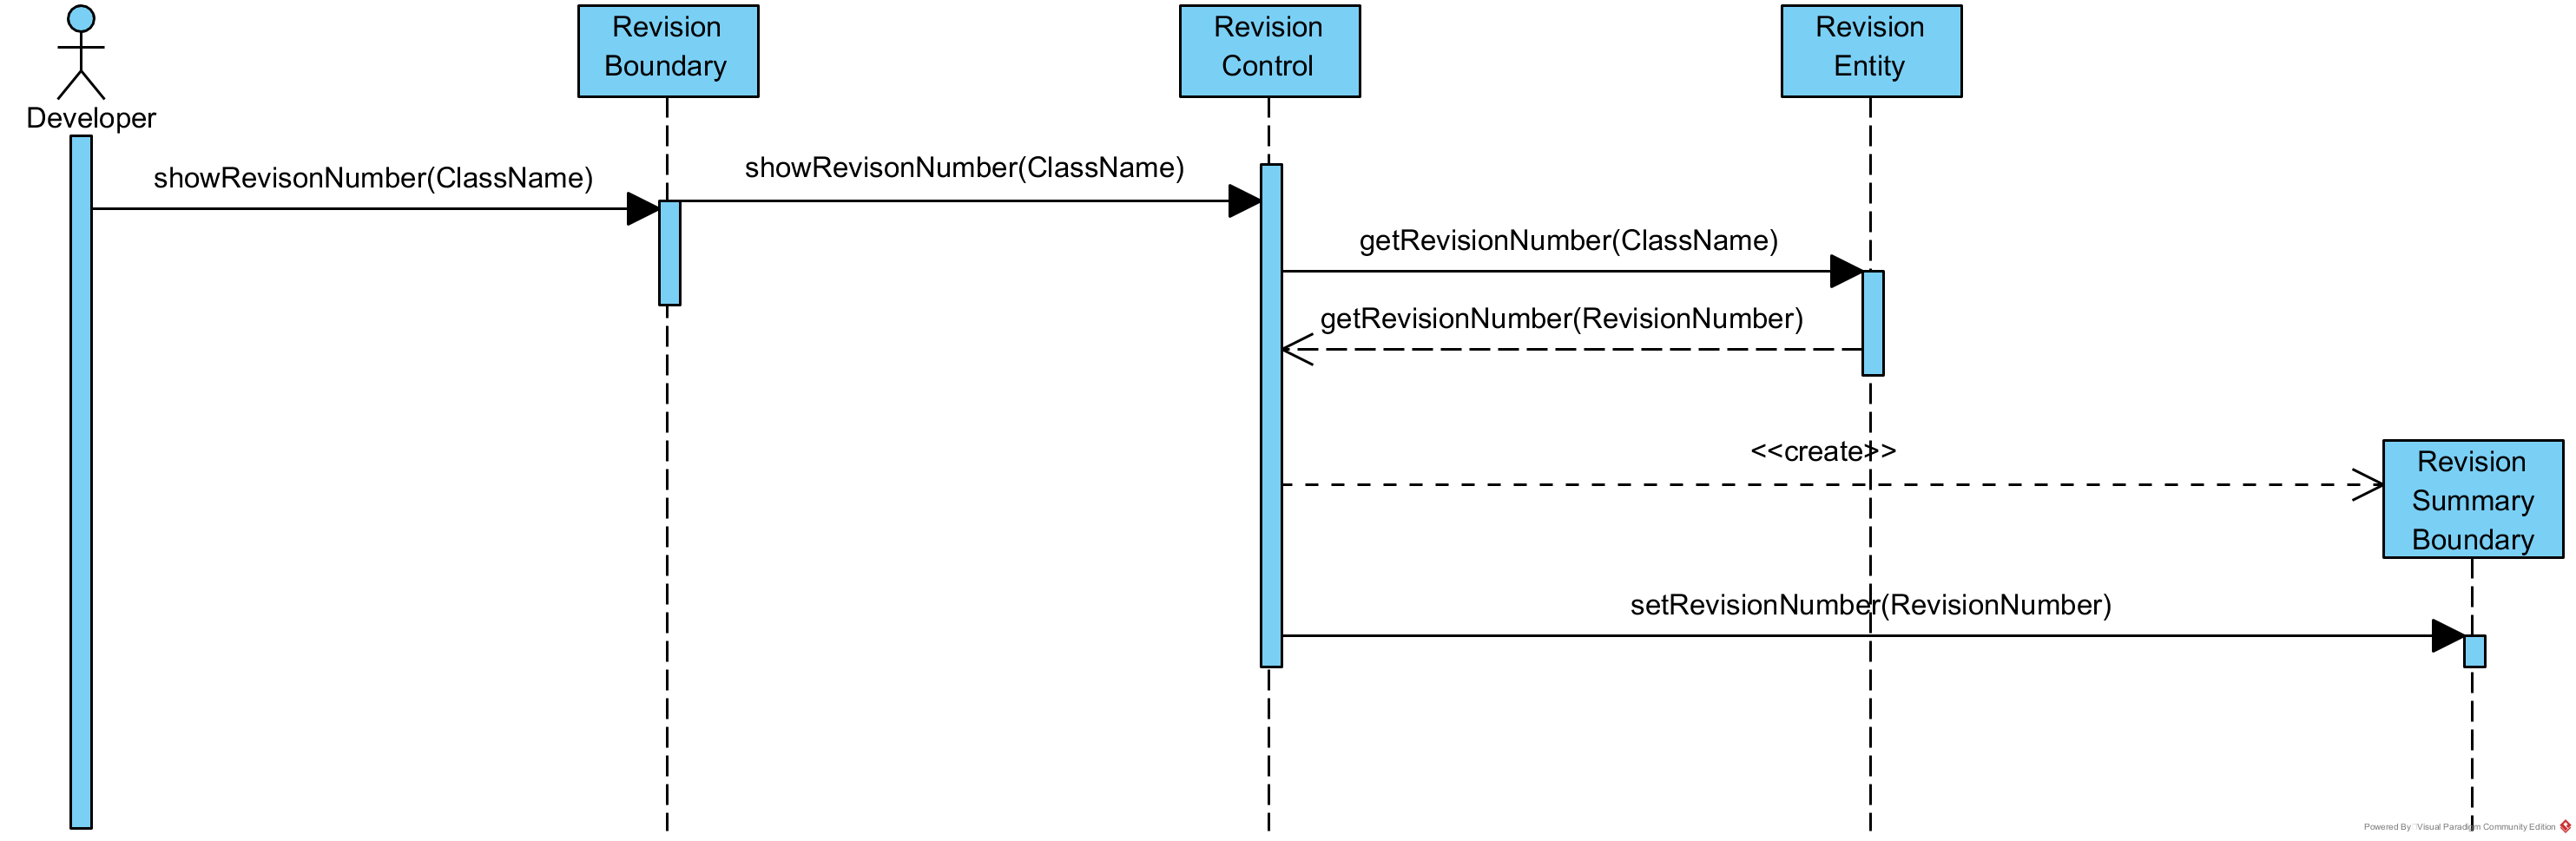
\includegraphics[width=\columnwidth]{LP_RevisionN.png}
    		\centering{SD2.9-Numero di modifiche e revisioni}
    	
    		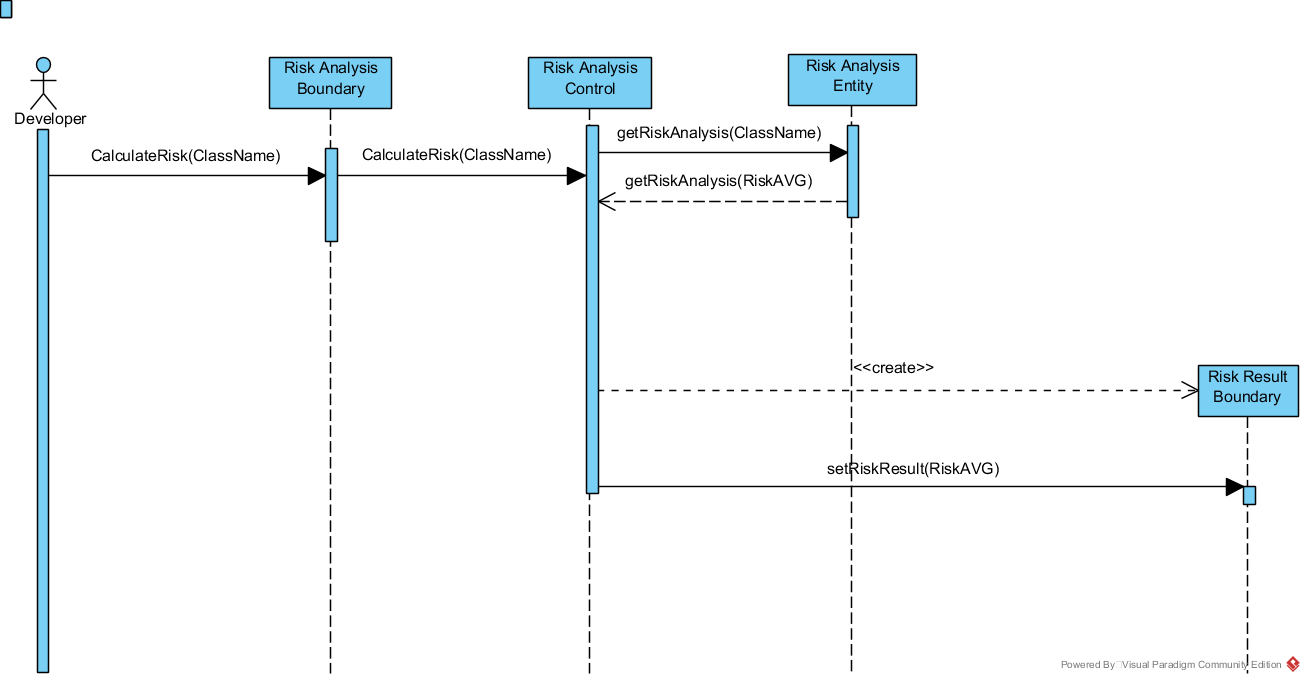
\includegraphics[width=\columnwidth]{LP_RiskAnalysis.png}
    		\centering{SD2.10-Analisi rischi}
	 
	  \flushleft
		\subsubsection{Activity Diagram}
		
			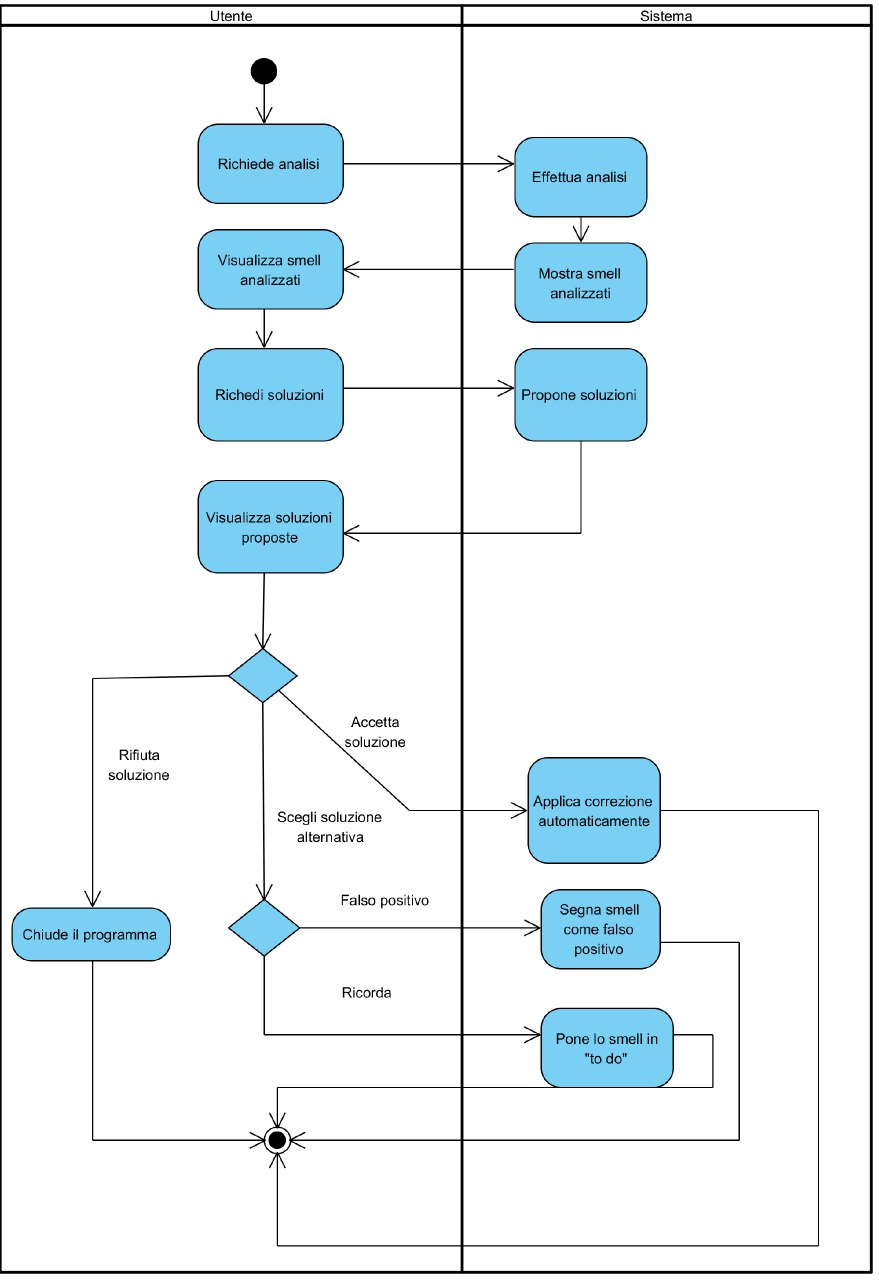
\includegraphics[width=\columnwidth]{ActivityDiagramProposed.jpg}
			\centering{AD1-Analisi, Correzione e Casi Opzionali di "Misplaced Class" e "Feature Envy"}
			\\
			\vspace{0.5cm}
			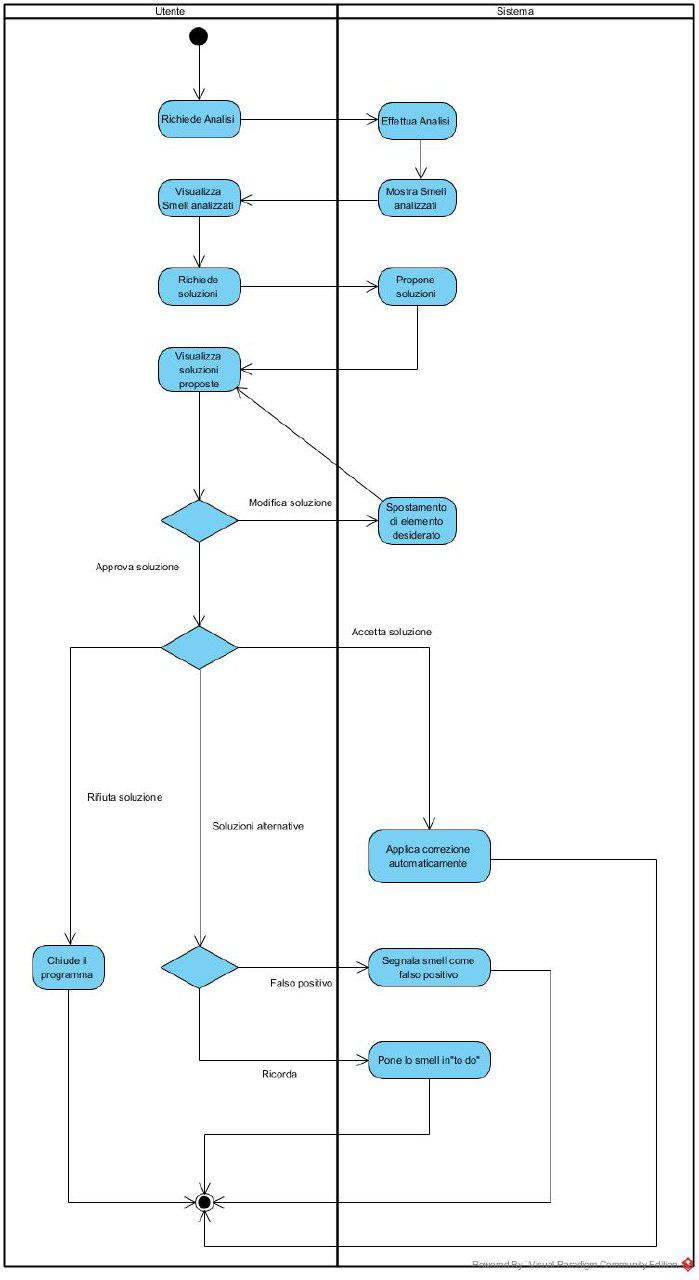
\includegraphics[width=\columnwidth]{ActivityDiagramProposedSwap.jpg}
			\centering{AD2-Analisi, Correzione e Casi Opzionali di "Blob" e "Promiscuous Package"}
			
	  \flushleft
		\subsubsection{New interface mockups}
		
			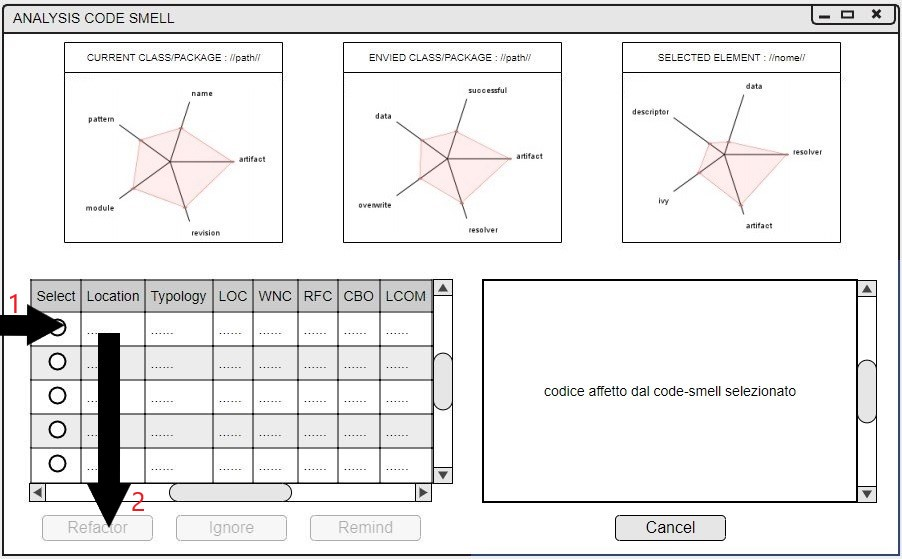
\includegraphics[width=\columnwidth]{mock-up_analisi1.jpg}
			\centering{MU1.1-Analisi}
			
			\flushleft
			L'utente, nel passo 1, seleziona nella tabella lo smell desiderato e visualizza automaticamente le 3 RadarMaps e la porzione di codice collegate. Prima della selezione i pulsanti risultano disabilitati.
			\\ \vspace{0.2cm}
			Tale schermata è collegata alla selezione nella tabella di code smell di tipo "Feature Envy" e "Misplaced Class". Nel caso di "Blob" e "Promiscuous Package" i pulsanti "Ignore" e "Remind" rimangono disabilitati e si viene rimandati a MU4.1 e successivi.
			\\\vspace{0.5cm}
			L'utente, nel passo 2, selezionando il pulsante "Refactoring" richiede la proposta di soluzione allo smell selezionato.\\ \vspace{0.5cm}
		
			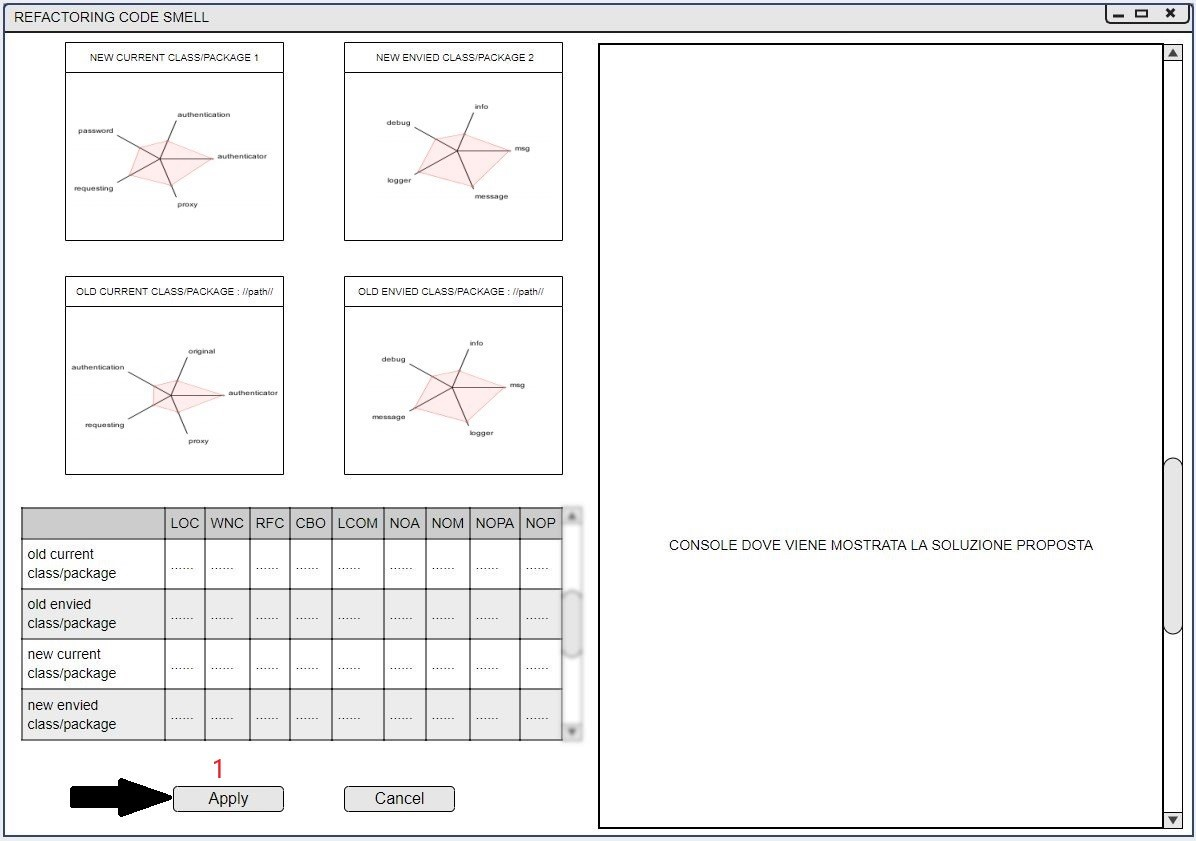
\includegraphics[width=\columnwidth]{mock-up_refactoring.jpg}
			\centering{MU1.2-Refactoring "Feature Envy" e "Misplaced Class"}
		
			\flushleft
			L'utente, nel passo 1, selezionando il pulsante "Apply" richiede l'applicazione della proposta di soluzione.\vspace{0.5cm}
		
			\centering
			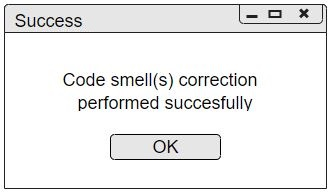
\includegraphics[scale=0.9]{pop-up_successo.jpg}\\
			\centering{MU1.3-Pop-up di successo}
			\vspace{0.5cm}
			
			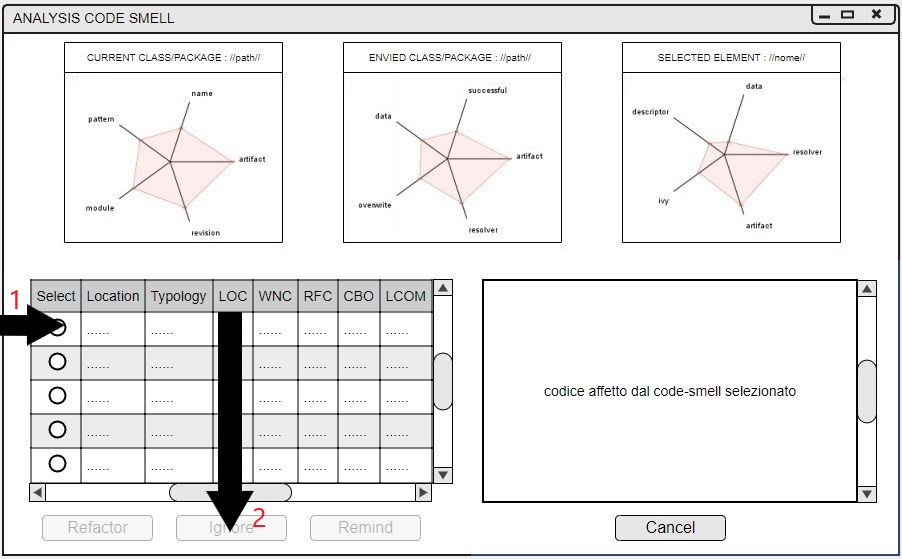
\includegraphics[width=\columnwidth]{mock-up_analisi2.jpg}
			\centering{MU2.1-Analisi}
			
			\flushleft
			L'utente, nel passo 1, seleziona nella tabella lo smell desiderato e visualizza automaticamente le 3 RadarMaps e la porzione di codice collegate.\\ \vspace{0.2cm}
			L'utente, nel passo 2, selezionando il pulsante "Ignore" richiede di ignorare lo smell selezionato.\vspace{0.5cm}
			
			\centering	
			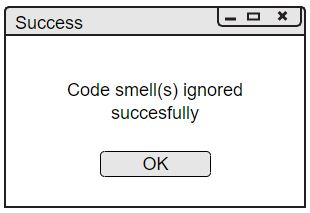
\includegraphics[scale=0.9]{pop_up_ignore.jpg}\\
			\centering{MU2.2-Pop-up ignora}
			
			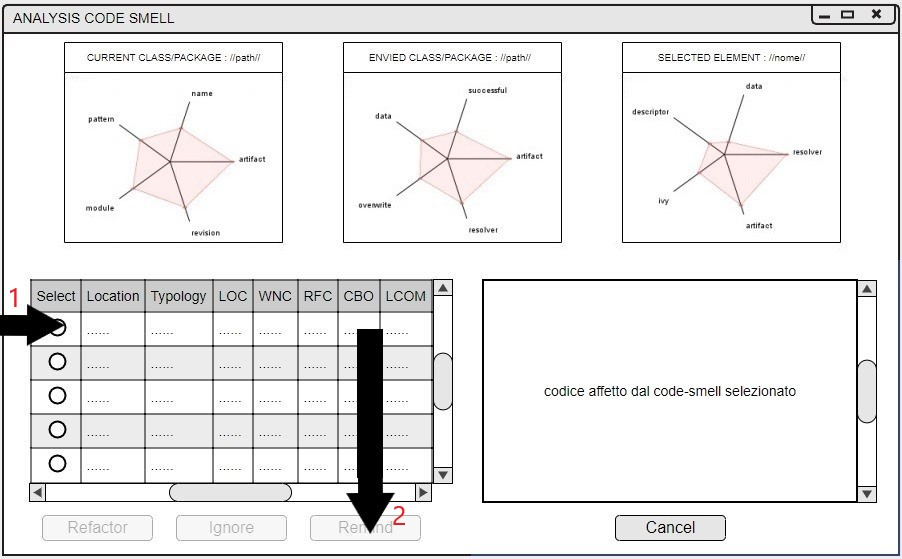
\includegraphics[width=\columnwidth]{mock-up_analisi3.jpg}
			\centering{MU3.1-Analisi}
			
			\flushleft
			L'utente, nel passo 1, seleziona nella tabella lo smell desiderato e visualizza automaticamente le 3 RadarMaps e la porzione di codice collegate.\\ \vspace{0.2cm}
			L'utente, nel passo 2, selezionando il pulsante "Remind" richiede di ricordare lo smell selezionato ed aggiungerlo alla lista "to do".\vspace{0.5cm}
			
			\centering	
			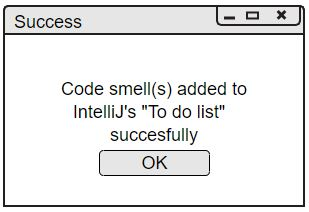
\includegraphics[scale=0.9]{pop-up_remind.jpg}\\
			\centering{MU3.2-Pop-up remind}
			
			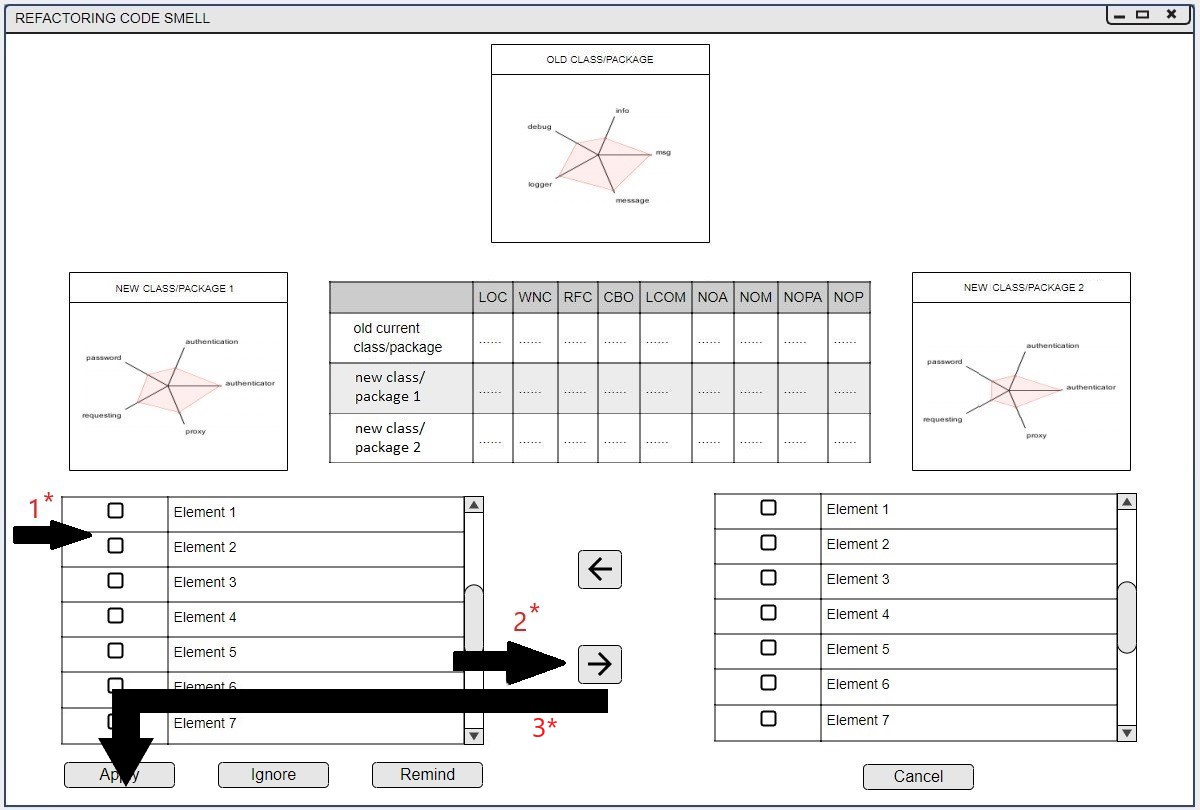
\includegraphics[width=\columnwidth]{mock-up_refactoring2_1.jpg}
			\centering{MU4.1-Refactoring "Blob" e "Promiscuous Package"}
			
			\flushleft
			L'utente, nel passo 1, selezionando una o più riga nella tabella e successivamente (tramite passo 2) premendo su apposito pulsante si effettua lo spostamento degli elementi selezionati nell'altra tabella. Tale operazione può essere effettuata anche sulla tabella di destra con la stessa logica.\vspace{0.2cm}
			\\L'utente, nel passo 3, selezionando il pulsante "Apply" richiede l'applicazione della proposta di soluzione.\vspace{0.3cm}
			
			*=identifica una operazione opzionale che può quindi essere anche non effettuata.
			\vspace{0.5cm}
			
			\centering	
			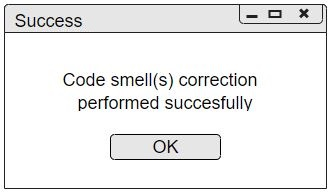
\includegraphics[scale=0.9]{pop-up_successo.jpg}\\
			\centering{MU4.2-Pop-up di successo}	
			
			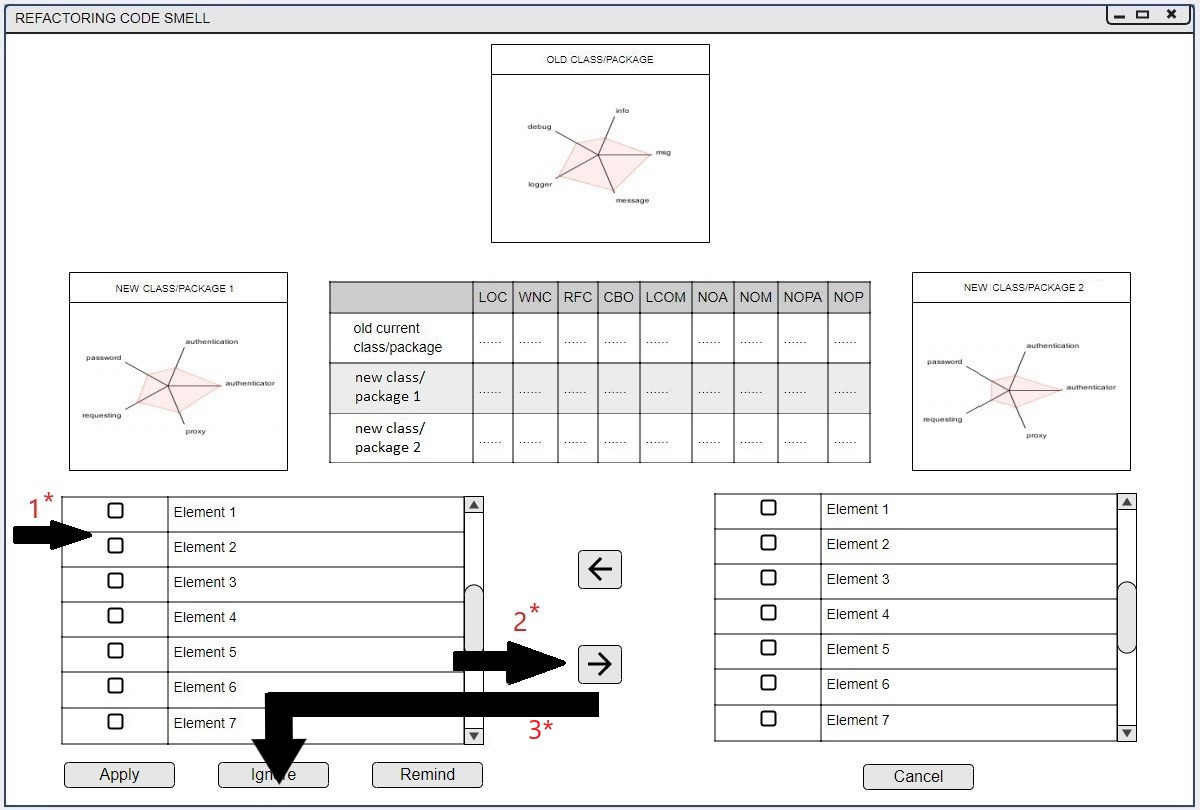
\includegraphics[width=\columnwidth]{mock-up_refactoring2_2.jpg}
			\centering{MU5.1-Refactoring seconda schermata}
			
			\flushleft
			L'utente, nel passo 1, selezionando una o più riga nella tabella e successivamente (tramite passo 2) premendo su apposito pulsante si effettua lo spostamento degli elementi selezionati nell'altra tabella. Tale operazione può essere effettuata anche sulla tabella di destra con la stessa logica.\vspace{0.2cm}
			\\L'utente, nel passo 3, selezionando il pulsante "Ignore" richiede di ignorare lo smell selezionato.\vspace{0.3cm}
			
			*=identifica una operazione opzionale che può quindi essere anche non effettuata.
			\vspace{0.5cm}
			
			\centering	
			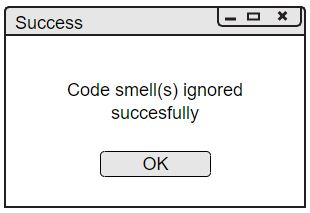
\includegraphics[scale=0.9]{pop_up_ignore.jpg}\\
			\centering{MU5.2-Pop-up ignora}
			
			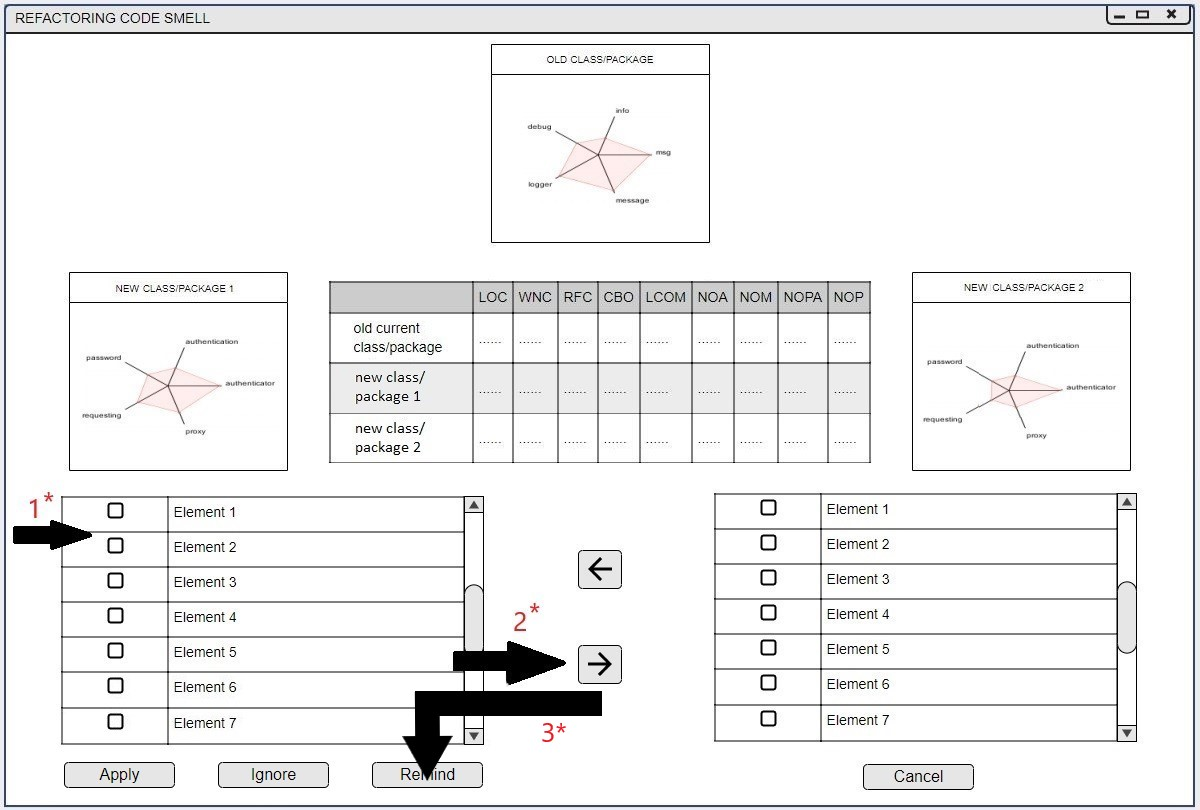
\includegraphics[width=\columnwidth]{mock-up_refactoring2_3.jpg}
			\centering{MU6.1-Refactoring seconda schermata}
			
			\flushleft
			L'utente, nel passo 1, selezionando una o più riga nella tabella e successivamente (tramite passo 2) premendo su apposito pulsante si effettua lo spostamento degli elementi selezionati nell'altra tabella. Tale operazione può essere effettuata anche sulla tabella di destra con la stessa logica.
			\\L'utente, nel passo 3, selezionando il pulsante "Remind"  richiede di ricordare lo smell selezionato ed aggiungerlo alla lista "to do".\vspace{0.2cm}
			
			*=identifica una operazione opzionale che può quindi essere anche non effettuata.
			\vspace{0.5cm}
			
			\centering	
			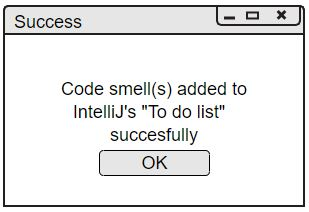
\includegraphics[scale=0.9]{pop-up_remind.jpg}\\
			\centering{MU6.2-Pop-up remind}
						
		\flushleft	
		\section{Glossary}
		
	   		
\begin{itemize}
	   			
	   			\item \textbf{Blob:} Tipoligia di code smell. E' una Classe che implementa responsabilità molto diverse tra di loro.
	   			
	   			\item \textbf{Feature Envy:} Tipoligia di code smell. E' un Metodo che è maggiormente interessato a variabili e metodi di una classe differente dalla sua.
	   			
	   			\item \textbf{IntelliJ IDEA:} IntelliJ IDEA è un ambiente di sviluppo integrato per il linguaggio di programmazione Java. E' stato sviluppato da JetBrains.
	   			
	   			\item \textbf{Misplaced Class:} Tipoligia di code smell. E' una Classe che non ha alcuna attinenza con le classi dello stesso package.
	   			
	   			\item \textbf{Promiscuous Package:} Tipoligia di code smell. E' un Package contenente classi che hanno responsabilità diverse.
	   			
	   			\item \textbf{TACOR:} Acronimo per Textual Analysis for Code smell detectiOn and Refactoring. E' un plug-in, sviluppato per l'IDE IntelliJ IDEA, creato per risolvere il problema dei "code smell" mediante l'analisi testuale. Esso è il progetto su cui è basato ASCETIC.
	   			
\end{itemize}

		
	
\end{document}
